\documentclass[11pt, oneside]{book}
%********************************************

\usepackage[phd]{thesisfrontmatter}
%\usepackage[proposal]{thesisfrontmatter}
% For Proposal, uncomment the line "\usepackage[proposal]{thesisfrontmatter}"

%%%%% NEW MATH DEFINITIONS %%%%%

\usepackage{amsmath}
\usepackage{amsfonts}
\usepackage{bm}

% Mark sections of captions for referring to divisions of figures
\newcommand{\figleft}{{\em (Left)}}
\newcommand{\figcenter}{{\em (Center)}}
\newcommand{\figright}{{\em (Right)}}
\newcommand{\figtop}{{\em (Top)}}
\newcommand{\figbottom}{{\em (Bottom)}}
\newcommand{\captiona}{{\em (a)}}
\newcommand{\captionb}{{\em (b)}}
\newcommand{\captionc}{{\em (c)}}
\newcommand{\captiond}{{\em (d)}}

% Highlight a newly defined term
\newcommand{\newterm}[1]{{\bf #1}}


% Figure reference, lower-case.
\def\figref#1{figure~\ref{#1}}
% Figure reference, capital. For start of sentence
\def\Figref#1{Figure~\ref{#1}}
\def\twofigref#1#2{figures \ref{#1} and \ref{#2}}
\def\quadfigref#1#2#3#4{figures \ref{#1}, \ref{#2}, \ref{#3} and \ref{#4}}
% Section reference, lower-case.
\def\secref#1{section~\ref{#1}}
% Section reference, capital.
\def\Secref#1{Section~\ref{#1}}
% Reference to two sections.
\def\twosecrefs#1#2{sections \ref{#1} and \ref{#2}}
% Reference to three sections.
\def\secrefs#1#2#3{sections \ref{#1}, \ref{#2} and \ref{#3}}
% Reference to an equation, lower-case.
\def\eqref#1{equation~\ref{#1}}
% Reference to an equation, upper case
\def\Eqref#1{Equation~\ref{#1}}
% A raw reference to an equation---avoid using if possible
\def\plaineqref#1{\ref{#1}}
% Reference to a chapter, lower-case.
\def\chapref#1{chapter~\ref{#1}}
% Reference to an equation, upper case.
\def\Chapref#1{Chapter~\ref{#1}}
% Reference to a range of chapters
\def\rangechapref#1#2{chapters\ref{#1}--\ref{#2}}
% Reference to an algorithm, lower-case.
\def\algref#1{algorithm~\ref{#1}}
% Reference to an algorithm, upper case.
\def\Algref#1{Algorithm~\ref{#1}}
\def\twoalgref#1#2{algorithms \ref{#1} and \ref{#2}}
\def\Twoalgref#1#2{Algorithms \ref{#1} and \ref{#2}}
% Reference to a part, lower case
\def\partref#1{part~\ref{#1}}
% Reference to a part, upper case
\def\Partref#1{Part~\ref{#1}}
\def\twopartref#1#2{parts \ref{#1} and \ref{#2}}

\def\ceil#1{\lceil #1 \rceil}
\def\floor#1{\lfloor #1 \rfloor}
\def\1{\bm{1}}
\newcommand{\train}{\mathcal{D}}
\newcommand{\valid}{\mathcal{D_{\mathrm{valid}}}}
\newcommand{\test}{\mathcal{D_{\mathrm{test}}}}

\def\eps{{\epsilon}}


% Random variables
\def\reta{{\textnormal{$\eta$}}}
\def\ra{{\textnormal{a}}}
\def\rb{{\textnormal{b}}}
\def\rc{{\textnormal{c}}}
\def\rd{{\textnormal{d}}}
\def\re{{\textnormal{e}}}
\def\rf{{\textnormal{f}}}
\def\rg{{\textnormal{g}}}
\def\rh{{\textnormal{h}}}
\def\ri{{\textnormal{i}}}
\def\rj{{\textnormal{j}}}
\def\rk{{\textnormal{k}}}
\def\rl{{\textnormal{l}}}
% rm is already a command, just don't name any random variables m
\def\rn{{\textnormal{n}}}
\def\ro{{\textnormal{o}}}
\def\rp{{\textnormal{p}}}
\def\rq{{\textnormal{q}}}
\def\rr{{\textnormal{r}}}
\def\rs{{\textnormal{s}}}
\def\rt{{\textnormal{t}}}
\def\ru{{\textnormal{u}}}
\def\rv{{\textnormal{v}}}
\def\rw{{\textnormal{w}}}
\def\rx{{\textnormal{x}}}
\def\ry{{\textnormal{y}}}
\def\rz{{\textnormal{z}}}

% Random vectors
\def\rvepsilon{{\mathbf{\epsilon}}}
\def\rvtheta{{\mathbf{\theta}}}
\def\rva{{\mathbf{a}}}
\def\rvb{{\mathbf{b}}}
\def\rvc{{\mathbf{c}}}
\def\rvd{{\mathbf{d}}}
\def\rve{{\mathbf{e}}}
\def\rvf{{\mathbf{f}}}
\def\rvg{{\mathbf{g}}}
\def\rvh{{\mathbf{h}}}
\def\rvu{{\mathbf{i}}}
\def\rvj{{\mathbf{j}}}
\def\rvk{{\mathbf{k}}}
\def\rvl{{\mathbf{l}}}
\def\rvm{{\mathbf{m}}}
\def\rvn{{\mathbf{n}}}
\def\rvo{{\mathbf{o}}}
\def\rvp{{\mathbf{p}}}
\def\rvq{{\mathbf{q}}}
\def\rvr{{\mathbf{r}}}
\def\rvs{{\mathbf{s}}}
\def\rvt{{\mathbf{t}}}
\def\rvu{{\mathbf{u}}}
\def\rvv{{\mathbf{v}}}
\def\rvw{{\mathbf{w}}}
\def\rvx{{\mathbf{x}}}
\def\rvy{{\mathbf{y}}}
\def\rvz{{\mathbf{z}}}

% Elements of random vectors
\def\erva{{\textnormal{a}}}
\def\ervb{{\textnormal{b}}}
\def\ervc{{\textnormal{c}}}
\def\ervd{{\textnormal{d}}}
\def\erve{{\textnormal{e}}}
\def\ervf{{\textnormal{f}}}
\def\ervg{{\textnormal{g}}}
\def\ervh{{\textnormal{h}}}
\def\ervi{{\textnormal{i}}}
\def\ervj{{\textnormal{j}}}
\def\ervk{{\textnormal{k}}}
\def\ervl{{\textnormal{l}}}
\def\ervm{{\textnormal{m}}}
\def\ervn{{\textnormal{n}}}
\def\ervo{{\textnormal{o}}}
\def\ervp{{\textnormal{p}}}
\def\ervq{{\textnormal{q}}}
\def\ervr{{\textnormal{r}}}
\def\ervs{{\textnormal{s}}}
\def\ervt{{\textnormal{t}}}
\def\ervu{{\textnormal{u}}}
\def\ervv{{\textnormal{v}}}
\def\ervw{{\textnormal{w}}}
\def\ervx{{\textnormal{x}}}
\def\ervy{{\textnormal{y}}}
\def\ervz{{\textnormal{z}}}

% Random matrices
\def\rmA{{\mathbf{A}}}
\def\rmB{{\mathbf{B}}}
\def\rmC{{\mathbf{C}}}
\def\rmD{{\mathbf{D}}}
\def\rmE{{\mathbf{E}}}
\def\rmF{{\mathbf{F}}}
\def\rmG{{\mathbf{G}}}
\def\rmH{{\mathbf{H}}}
\def\rmI{{\mathbf{I}}}
\def\rmJ{{\mathbf{J}}}
\def\rmK{{\mathbf{K}}}
\def\rmL{{\mathbf{L}}}
\def\rmM{{\mathbf{M}}}
\def\rmN{{\mathbf{N}}}
\def\rmO{{\mathbf{O}}}
\def\rmP{{\mathbf{P}}}
\def\rmQ{{\mathbf{Q}}}
\def\rmR{{\mathbf{R}}}
\def\rmS{{\mathbf{S}}}
\def\rmT{{\mathbf{T}}}
\def\rmU{{\mathbf{U}}}
\def\rmV{{\mathbf{V}}}
\def\rmW{{\mathbf{W}}}
\def\rmX{{\mathbf{X}}}
\def\rmY{{\mathbf{Y}}}
\def\rmZ{{\mathbf{Z}}}

% Elements of random matrices
\def\ermA{{\textnormal{A}}}
\def\ermB{{\textnormal{B}}}
\def\ermC{{\textnormal{C}}}
\def\ermD{{\textnormal{D}}}
\def\ermE{{\textnormal{E}}}
\def\ermF{{\textnormal{F}}}
\def\ermG{{\textnormal{G}}}
\def\ermH{{\textnormal{H}}}
\def\ermI{{\textnormal{I}}}
\def\ermJ{{\textnormal{J}}}
\def\ermK{{\textnormal{K}}}
\def\ermL{{\textnormal{L}}}
\def\ermM{{\textnormal{M}}}
\def\ermN{{\textnormal{N}}}
\def\ermO{{\textnormal{O}}}
\def\ermP{{\textnormal{P}}}
\def\ermQ{{\textnormal{Q}}}
\def\ermR{{\textnormal{R}}}
\def\ermS{{\textnormal{S}}}
\def\ermT{{\textnormal{T}}}
\def\ermU{{\textnormal{U}}}
\def\ermV{{\textnormal{V}}}
\def\ermW{{\textnormal{W}}}
\def\ermX{{\textnormal{X}}}
\def\ermY{{\textnormal{Y}}}
\def\ermZ{{\textnormal{Z}}}

% Vectors
\def\vzero{{\bm{0}}}
\def\vone{{\bm{1}}}
\def\vmu{{\bm{\mu}}}
\def\vtheta{{\bm{\theta}}}
\def\va{{\bm{a}}}
\def\vb{{\bm{b}}}
\def\vc{{\bm{c}}}
\def\vd{{\bm{d}}}
\def\ve{{\bm{e}}}
\def\vf{{\bm{f}}}
\def\vg{{\bm{g}}}
\def\vh{{\bm{h}}}
\def\vi{{\bm{i}}}
\def\vj{{\bm{j}}}
\def\vk{{\bm{k}}}
\def\vl{{\bm{l}}}
\def\vm{{\bm{m}}}
\def\vn{{\bm{n}}}
\def\vo{{\bm{o}}}
\def\vp{{\bm{p}}}
\def\vq{{\bm{q}}}
\def\vr{{\bm{r}}}
\def\vs{{\bm{s}}}
\def\vt{{\bm{t}}}
\def\vu{{\bm{u}}}
\def\vv{{\bm{v}}}
\def\vw{{\bm{w}}}
\def\vx{{\bm{x}}}
\def\vy{{\bm{y}}}
\def\vz{{\bm{z}}}

% Elements of vectors
\def\evalpha{{\alpha}}
\def\evbeta{{\beta}}
\def\evepsilon{{\epsilon}}
\def\evlambda{{\lambda}}
\def\evomega{{\omega}}
\def\evmu{{\mu}}
\def\evpsi{{\psi}}
\def\evsigma{{\sigma}}
\def\evtheta{{\theta}}
\def\eva{{a}}
\def\evb{{b}}
\def\evc{{c}}
\def\evd{{d}}
\def\eve{{e}}
\def\evf{{f}}
\def\evg{{g}}
\def\evh{{h}}
\def\evi{{i}}
\def\evj{{j}}
\def\evk{{k}}
\def\evl{{l}}
\def\evm{{m}}
\def\evn{{n}}
\def\evo{{o}}
\def\evp{{p}}
\def\evq{{q}}
\def\evr{{r}}
\def\evs{{s}}
\def\evt{{t}}
\def\evu{{u}}
\def\evv{{v}}
\def\evw{{w}}
\def\evx{{x}}
\def\evy{{y}}
\def\evz{{z}}

% Matrix
\def\mA{{\bm{A}}}
\def\mB{{\bm{B}}}
\def\mC{{\bm{C}}}
\def\mD{{\bm{D}}}
\def\mE{{\bm{E}}}
\def\mF{{\bm{F}}}
\def\mG{{\bm{G}}}
\def\mH{{\bm{H}}}
\def\mI{{\bm{I}}}
\def\mJ{{\bm{J}}}
\def\mK{{\bm{K}}}
\def\mL{{\bm{L}}}
\def\mM{{\bm{M}}}
\def\mN{{\bm{N}}}
\def\mO{{\bm{O}}}
\def\mP{{\bm{P}}}
\def\mQ{{\bm{Q}}}
\def\mR{{\bm{R}}}
\def\mS{{\bm{S}}}
\def\mT{{\bm{T}}}
\def\mU{{\bm{U}}}
\def\mV{{\bm{V}}}
\def\mW{{\bm{W}}}
\def\mX{{\bm{X}}}
\def\mY{{\bm{Y}}}
\def\mZ{{\bm{Z}}}
\def\mBeta{{\bm{\beta}}}
\def\mPhi{{\bm{\Phi}}}
\def\mLambda{{\bm{\Lambda}}}
\def\mSigma{{\bm{\Sigma}}}

% Tensor
\DeclareMathAlphabet{\mathsfit}{\encodingdefault}{\sfdefault}{m}{sl}
\SetMathAlphabet{\mathsfit}{bold}{\encodingdefault}{\sfdefault}{bx}{n}
\newcommand{\tens}[1]{\bm{\mathsfit{#1}}}
\def\tA{{\tens{A}}}
\def\tB{{\tens{B}}}
\def\tC{{\tens{C}}}
\def\tD{{\tens{D}}}
\def\tE{{\tens{E}}}
\def\tF{{\tens{F}}}
\def\tG{{\tens{G}}}
\def\tH{{\tens{H}}}
\def\tI{{\tens{I}}}
\def\tJ{{\tens{J}}}
\def\tK{{\tens{K}}}
\def\tL{{\tens{L}}}
\def\tM{{\tens{M}}}
\def\tN{{\tens{N}}}
\def\tO{{\tens{O}}}
\def\tP{{\tens{P}}}
\def\tQ{{\tens{Q}}}
\def\tR{{\tens{R}}}
\def\tS{{\tens{S}}}
\def\tT{{\tens{T}}}
\def\tU{{\tens{U}}}
\def\tV{{\tens{V}}}
\def\tW{{\tens{W}}}
\def\tX{{\tens{X}}}
\def\tY{{\tens{Y}}}
\def\tZ{{\tens{Z}}}


% Graph
\def\gA{{\mathcal{A}}}
\def\gB{{\mathcal{B}}}
\def\gC{{\mathcal{C}}}
\def\gD{{\mathcal{D}}}
\def\gE{{\mathcal{E}}}
\def\gF{{\mathcal{F}}}
\def\gG{{\mathcal{G}}}
\def\gH{{\mathcal{H}}}
\def\gI{{\mathcal{I}}}
\def\gJ{{\mathcal{J}}}
\def\gK{{\mathcal{K}}}
\def\gL{{\mathcal{L}}}
\def\gM{{\mathcal{M}}}
\def\gN{{\mathcal{N}}}
\def\gO{{\mathcal{O}}}
\def\gP{{\mathcal{P}}}
\def\gQ{{\mathcal{Q}}}
\def\gR{{\mathcal{R}}}
\def\gS{{\mathcal{S}}}
\def\gT{{\mathcal{T}}}
\def\gU{{\mathcal{U}}}
\def\gV{{\mathcal{V}}}
\def\gW{{\mathcal{W}}}
\def\gX{{\mathcal{X}}}
\def\gY{{\mathcal{Y}}}
\def\gZ{{\mathcal{Z}}}

% Sets
\def\sA{{\mathbb{A}}}
\def\sB{{\mathbb{B}}}
\def\sC{{\mathbb{C}}}
\def\sD{{\mathbb{D}}}
% Don't use a set called E, because this would be the same as our symbol
% for expectation.
\def\sF{{\mathbb{F}}}
\def\sG{{\mathbb{G}}}
\def\sH{{\mathbb{H}}}
\def\sI{{\mathbb{I}}}
\def\sJ{{\mathbb{J}}}
\def\sK{{\mathbb{K}}}
\def\sL{{\mathbb{L}}}
\def\sM{{\mathbb{M}}}
\def\sN{{\mathbb{N}}}
\def\sO{{\mathbb{O}}}
\def\sP{{\mathbb{P}}}
\def\sQ{{\mathbb{Q}}}
\def\sR{{\mathbb{R}}}
\def\sS{{\mathbb{S}}}
\def\sT{{\mathbb{T}}}
\def\sU{{\mathbb{U}}}
\def\sV{{\mathbb{V}}}
\def\sW{{\mathbb{W}}}
\def\sX{{\mathbb{X}}}
\def\sY{{\mathbb{Y}}}
\def\sZ{{\mathbb{Z}}}

% Entries of a matrix
\def\emLambda{{\Lambda}}
\def\emA{{A}}
\def\emB{{B}}
\def\emC{{C}}
\def\emD{{D}}
\def\emE{{E}}
\def\emF{{F}}
\def\emG{{G}}
\def\emH{{H}}
\def\emI{{I}}
\def\emJ{{J}}
\def\emK{{K}}
\def\emL{{L}}
\def\emM{{M}}
\def\emN{{N}}
\def\emO{{O}}
\def\emP{{P}}
\def\emQ{{Q}}
\def\emR{{R}}
\def\emS{{S}}
\def\emT{{T}}
\def\emU{{U}}
\def\emV{{V}}
\def\emW{{W}}
\def\emX{{X}}
\def\emY{{Y}}
\def\emZ{{Z}}
\def\emSigma{{\Sigma}}

% entries of a tensor
% Same font as tensor, without \bm wrapper
\newcommand{\etens}[1]{\mathsfit{#1}}
\def\etLambda{{\etens{\Lambda}}}
\def\etA{{\etens{A}}}
\def\etB{{\etens{B}}}
\def\etC{{\etens{C}}}
\def\etD{{\etens{D}}}
\def\etE{{\etens{E}}}
\def\etF{{\etens{F}}}
\def\etG{{\etens{G}}}
\def\etH{{\etens{H}}}
\def\etI{{\etens{I}}}
\def\etJ{{\etens{J}}}
\def\etK{{\etens{K}}}
\def\etL{{\etens{L}}}
\def\etM{{\etens{M}}}
\def\etN{{\etens{N}}}
\def\etO{{\etens{O}}}
\def\etP{{\etens{P}}}
\def\etQ{{\etens{Q}}}
\def\etR{{\etens{R}}}
\def\etS{{\etens{S}}}
\def\etT{{\etens{T}}}
\def\etU{{\etens{U}}}
\def\etV{{\etens{V}}}
\def\etW{{\etens{W}}}
\def\etX{{\etens{X}}}
\def\etY{{\etens{Y}}}
\def\etZ{{\etens{Z}}}

% The true underlying data generating distribution
\newcommand{\pdata}{p_{\rm{data}}}
% The empirical distribution defined by the training set
\newcommand{\ptrain}{\hat{p}_{\rm{data}}}
\newcommand{\Ptrain}{\hat{P}_{\rm{data}}}
% The model distribution
\newcommand{\pmodel}{p_{\rm{model}}}
\newcommand{\Pmodel}{P_{\rm{model}}}
\newcommand{\ptildemodel}{\tilde{p}_{\rm{model}}}
% Stochastic autoencoder distributions
\newcommand{\pencode}{p_{\rm{encoder}}}
\newcommand{\pdecode}{p_{\rm{decoder}}}
\newcommand{\precons}{p_{\rm{reconstruct}}}

\newcommand{\laplace}{\mathrm{Laplace}} % Laplace distribution

\newcommand{\E}{\mathbb{E}}
\newcommand{\Ls}{\mathcal{L}}
\newcommand{\R}{\mathbb{R}}
\newcommand{\emp}{\tilde{p}}
\newcommand{\lr}{\alpha}
\newcommand{\reg}{\lambda}
\newcommand{\rect}{\mathrm{rectifier}}
\newcommand{\softmax}{\mathrm{softmax}}
\newcommand{\sigmoid}{\sigma}
\newcommand{\softplus}{\zeta}
\newcommand{\KL}{D_{\mathrm{KL}}}
\newcommand{\Var}{\mathrm{Var}}
\newcommand{\standarderror}{\mathrm{SE}}
\newcommand{\Cov}{\mathrm{Cov}}
% Wolfram Mathworld says $L^2$ is for function spaces and $\ell^2$ is for vectors
% But then they seem to use $L^2$ for vectors throughout the site, and so does
% wikipedia.
\newcommand{\normlzero}{L^0}
\newcommand{\normlone}{L^1}
\newcommand{\normltwo}{L^2}
\newcommand{\normlp}{L^p}
\newcommand{\normmax}{L^\infty}

\newcommand{\parents}{Pa} % See usage in notation.tex. Chosen to match Daphne's book.

\DeclareMathOperator*{\argmax}{arg\,max}
\DeclareMathOperator*{\argmin}{arg\,min}

\DeclareMathOperator{\sign}{sign}
\DeclareMathOperator{\Tr}{Tr}
\let\ab\allowbreak


\newcommand{\cX}{\mathcal{X}}
\newcommand{\cD}{\mathcal{D}}


\setlength{\parindent}{0pt}
\usepackage{booktabs}
\usepackage{amsmath} % math extensions
\usepackage{amsfonts} %...and ams math fonts
\usepackage{multicol} % Allow spanning cells in tables
\usepackage{graphics} % .jpg, .png, .pdf image import 
% automatically sorts citations; comment to disable
\usepackage[sort,nocompress]{cite} 
\usepackage[toc,page]{appendix} % for appendices
% \usepackage[margin=1.0in]{geometry}
\usepackage{geometry}
\usepackage[hyphens]{url}
\usepackage{natbib}
% \usepackage{url}
\usepackage{graphicx}
\usepackage{subfigure}
\usepackage{booktabs} % for professional tables
% For theorems and such
\usepackage{amsmath}
\usepackage{amssymb}
\usepackage{mathtools}
\usepackage{amsthm}
\usepackage{placeins}
\theoremstyle{plain}
\newtheorem{theorem}{Theorem}[section]
\newtheorem{proposition}[theorem]{Proposition}
\newtheorem{lemma}[theorem]{Lemma}
\newtheorem{corollary}[theorem]{Corollary}
\theoremstyle{definition}
\newtheorem{definition}[theorem]{Definition}
\newtheorem{assumption}[theorem]{Assumption}
\newtheorem{method}[theorem]{Method}
\theoremstyle{remark}
\newtheorem{remark}[theorem]{Remark}
\usepackage{wrapfig} 
\usepackage{xcolor}
\usepackage{colortbl}
\usepackage{algorithm}
\usepackage{algpseudocode}
\begin{document}

%*******************************************
% FRONT MATTER
%*******************************************
\pagenumbering{roman}
\degreetitle{[Proposal Title {\bf OR} Dissertation Title as it appears on the Dissertation Certificate]}

\degreeauthor{[professional name of author]}

\degreedate{[Month and year of
Dissertation Acceptance was signed]}

%\prevdegreeA{B.S. Penn State University, 1994}

%\prevdegreeB{M.S. Stony Brook University, 1998}

\advisor{[Advisor's name]}

\memberA{[Committee member's name]}
\memberB{[Committee member's name]}
\memberC{[Committee member's name]}
\memberD{[Ph.D. Program Director name]}
\externalchair{[External Chair's name]}

%********************************************
% FOR PROPOSAL, uncomment the following lines
%\makeproposaldeclaration
%\makePHDproposalapproval

% FOR THESIS
\makedeclaration
\makeapproval
\makecopyright
%********************************************


\begin{abstract}
This is the abstract text with no more than 350 words.

\end{abstract}
\begin{acknowledgements}
This is the acknowledgements text
\end{acknowledgements}
\begin{dedication}

This is the dedication text
\end{dedication}

% TABLE OF CONTENTS + LISTS OF FIGS/TABLES
\tableofcontents
\listoffigures
\listoftables

% Hack: make sure arabic numerals start
% on first page of the introduction.
\pagebreak
\pagenumbering{arabic}

%*******************************************
% MAIN TEXT
%*******************************************

% Chapters of the document 
% (in separate .tex files)
\chapter{Introduction}

\chapter{Background and Definitions}

\section{Out of Distribution Detection}

Out-of-distribution (OOD) detection addresses a critical challenge in modern machine learning: the ability to recognize when a model is presented with inputs that fall outside the scope of what it has been trained to understand. While supervised models excel at making predictions within the distribution of their training data, they are notoriously prone to overconfident predictions when confronted with novel or unexpected inputs — sometimes with dangerous consequences, especially in high-stakes applications such as healthcare, autonomous driving, or security systems.

The task of out-of-distribution detection is to identify a semantic shift in the data \citep{yang2021generalized}. This is determining when no predicted label could match the true label $\vy \notin \sY_{in}$, where $\sY_{in}$ represents the set of in-distribution training labels. In this case, we would consider the semantic space of the sample and the training distribution to be different, representing a semantic shift. We can express the probability that a sample is out-of-distribution via $P(\vy \notin \sY_{in} | \vx)$. 

\begin{definition}
    Out-of-Distribution (OOD) Detection: Given an input $\rvx$ and a set of in-distribution labels $\sY_{\text{in}}$, OOD detection is the task of identifying whether the true label $\rvy$ belongs outside the in-distribution set, i.e., $\rvy \notin \sY_{\text{in}}$, or equivalently estimating $P(\rvy \notin \sY_{\text{in}} \mid \rvx)$.
    \label{defineood}
    \vspace{-2mm}
\end{definition}

One baseline approach to estimate this probability is the \textit{Maximum Softmax Probability (MSP)} method. Here, a trained classifier outputs softmax probabilities across known classes, and the maximum probability $\texttt{MSP}(\mathbf{x})$ is interpreted as a confidence score. A low maximum confidence suggests that the input might not belong to any known class, leading to the simple baseline:

\begin{method}[Maximum Softmax Probability (MSP)]
Given an input $\mathbf{x}$, the MSP method estimates the probability of being out-of-distribution as $1 - \texttt{MSP}(\mathbf{x})$, where $\texttt{MSP}(\mathbf{x}) = \max_{y \in \mathcal{Y}_{\text{in}}} P(y \mid \mathbf{x})$.
\label{methodmsp}
\end{method}

Furthermore, we are only concerned with labels that can be generated using only $\rvx$, via function $f$ which depends solely on $\rvx$ and no other information. $f_\rvy$ may represent human labelers that generate $\rvy$. If we consider $\sY_{all}$ as the set of all possible labels that can be generated from $f_\rvy(\rvx \in \sX_{all})$, a subset of $\sX_{all}$ considered as $\sX_{training}$ may not contain all labels in $\sY_{all}$. For real world datasets, it is possible that $\sY_{in} \subsetneq \sY_{all}$.



While related to other concepts like \textit{anomaly detection}, OOD detection is distinct in key ways. Anomaly detection usually focuses on rare or abnormal data points \textit{within} the same distribution (e.g., detecting fraudulent transactions), whereas OOD detection focuses on recognizing inputs from \textit{entirely different} distributions or classes, outside the model’s prior knowledge. Furthermore, OOD detection primarily targets \textit{epistemic uncertainty} — the model’s uncertainty due to limited knowledge — rather than \textit{aleatoric uncertainty}, which arises from inherent noise or variability in the data.

Practically, OOD detection methods fall into two broad categories:
\begin{itemize}
    \item \textbf{Training-agnostic approaches}, like MSP or entropy-based scoring, which apply directly to existing classifiers without altering their training process.
    \item \textbf{Training-aware approaches}, which adapt model architectures, loss functions, or data augmentation strategies specifically to improve OOD recognition capabilities.
\end{itemize}

Evaluation typically involves exposing the model to benchmark OOD datasets designed to test its ability to reject or abstain from confident predictions on unfamiliar samples, while maintaining strong performance on in-distribution data. Additional information regarding methods and benchmarks will be provided in a later section. 


\section{Anomaly Detection}

Although anomaly detection and out-of-distribution (OOD) detection are sometimes used interchangeably in the literature, they address fundamentally different problems, with distinct assumptions, goals, and evaluation settings.

\subsection{Definiton and Scope}

Anomaly detection focuses on identifying individual data points that deviate significantly from the expected patterns within a single dataset or distribution. These anomalies, or outliers, are typically rare and often correspond to noise, rare events, or fraudulent activities within the same domain as the training data. For example, anomaly detection might flag fraudulent transactions in a credit card dataset, where the system has only ever seen transaction records from that specific financial context.

OOD detection, on the other hand, aims to detect data that comes from a different distribution altogether — one that was not seen during training. It concerns the model’s ability to recognize when a test input belongs to a class, domain, or environment that falls outside the model’s learned distribution. For example, an image classifier trained only on animals should ideally flag an image of a car as OOD, even though the car is not necessarily anomalous within its own context.

\subsection{Training Assumptions}

Anomaly detection methods typically assume access only to normal (non-anomalous) data during training and must learn to recognize deviations without ever seeing examples of the anomalies. This is often referred to as a one-class learning problem.

In contrast, OOD detection typically operates in a supervised learning context where the model has been trained on multiple in-distribution classes, and the challenge is to detect test inputs that fall outside this known set. Here, the focus is on recognizing the model’s epistemic uncertainty — i.e., knowing what the model doesn’t know.

\subsection{Evaluation Settings}

Anomaly detection is typically evaluated using synthetic or labeled anomaly datasets, where the goal is to identify rare but known outlier patterns within the same dataset.

OOD detection is evaluated by exposing the model to entirely new datasets or domains and measuring its ability to correctly reject or abstain from making confident predictions on these unfamiliar inputs. This setting often requires curated OOD benchmark datasets distinct from the in-distribution training data.

\section{Information Theory}

Information theory provides a mathematical framework for quantifying uncertainty, information content, and the relationships between random variables. Originally developed by \citet{shannon1948mathematical}, it has become foundational for many areas of machine learning, including uncertainty quantification, representation learning, and out-of-distribution (OOD) detection. The following are various definitions that are critical to understanding information theory.


\begin{definition}
\textbf{Entropy}: The entropy of a discrete random variable $\rvx$ with distribution $p(\vx)$ is defined as the expected amount of uncertainty or information contained in $\rvx$, denoted by $H(\rvx)$.
\label{def:entropy}
\end{definition}

\begin{definition}
\textbf{Conditional Entropy}: The conditional entropy $H(\rvy \mid \rvx)$ measures the remaining uncertainty in a random variable $\rvy$ given knowledge of another random variable $\rvx$.
\label{def:conditional_entropy}
\end{definition}

\begin{definition}
\textbf{Mutual Information}: The mutual information between random variables $\rvx$ and $\rvy$, denoted $I(\rvx; \rvy)$, quantifies the amount of information shared between $\rvx$ and $\rvy$, or equivalently, the reduction in uncertainty about $\rvx$ given knowledge of $\rvy$.
\label{def:mutual_information}
\end{definition}

\begin{definition}
\textbf{Kullback-Leibler (KL) Divergence}: The KL divergence between two distributions $P$ and $Q$, denoted $D_{\mathrm{KL}}(P \parallel Q)$, measures how much the distribution $P$ diverges from the reference distribution $Q$.
\label{def:kl_divergence}
\end{definition}

\begin{definition}
\textbf{Chain Rule for Entropy}: The joint entropy of two random variables $\rvx$ and $\rvy$ satisfies the chain rule:
\[
H(\rvx, \rvy) = H(\rvx) + H(\rvy \mid \rvx),
\]
expressing that the total uncertainty can be decomposed into the uncertainty of $\rvx$ plus the uncertainty of $\rvy$ given $\rvx$.
\label{def:chain_rule}
\end{definition}

\begin{definition}
\textbf{Mutual Information as KL Divergence}: The mutual information between $\rvx$ and $\rvy$ can be equivalently defined as the KL divergence between the joint distribution $p(\vx, \vy)$ and the product of the marginals $p(\vx)p(\vy)$:
\[
I(\rvx; \rvy) = D_{\mathrm{KL}}(p(\vx, \vy) \parallel p(\vx)p(\vy)).
\]
\label{def:mi_kl}
\end{definition}

\begin{definition}
\textbf{Non-negativity of Mutual Information}: Mutual information is always non-negative, that is, $I(\rvx; \rvy) \geq 0$, with equality if and only if $\rvx$ and $\rvy$ are independent.
\label{def:nonneg_mi}
\end{definition}

\begin{definition}
\textbf{Chain Rule for Mutual Information}: The mutual information between two random variables $\rvx$ and $\rvy$ can be decomposed using the chain rule as follows:
\[
I(\rvx; \rvy) = I(\rvx; \rvz) + I(\rvz; \rvy \mid \rvx),
\]
where $\rvz$ is a third variable, and $I(\rvx; \rvy)$ represents the total mutual information between $\rvx$ and $\rvy$. This decomposition expresses the amount of shared information in terms of intermediate variables that mediate the relationship.
\label{def:chain_rule_mi}
\end{definition}

\subsection{Entropy and Mutual Information}

Entropy and mutual information are central concepts in information theory, and they play a key role in understanding uncertainty and information flow in machine learning models. 

\textbf{Entropy}, as defined in Definition \ref{def:entropy}, measures the average uncertainty in a random variable $\rvx$. It quantifies how much unpredictability exists in the outcomes of $\rvx$. In machine learning, entropy is often used to assess the uncertainty in a model's predictions or to regularize a model by minimizing its uncertainty.

\textbf{Mutual information}, as defined in Definition \ref{def:mutual_information}, measures the amount of information shared between two random variables, $\rvx$ and $\rvy$. Specifically, it quantifies how much knowing one variable reduces uncertainty about the other. In machine learning, mutual information is used to gauge the relevance of features to the target variable, aiding in feature selection and representation learning. By maximizing mutual information between representations and labels, we can improve the expressiveness and usefulness of learned features.

\section{Information Bottleneck and Minimal Sufficient Statistic}

In this section, we introduce two important concepts in information theory that are relevant for understanding how to efficiently represent information while preserving relevant information: the **Information Bottleneck** and the **Minimal Sufficient Statistic**.


\subsection{Minimal Sufficient Statistic}

A **Minimal Sufficient Statistic** is a concept from statistics that defines a statistic that captures all the information about a parameter of interest in a dataset while being the most compact representation. In the context of information theory, it is the statistic that minimizes the loss of information and is often used in maximum likelihood estimation (MLE).

\begin{definition}
\textbf{Minimal Sufficient Statistic}: A statistic \( T(\rvx) \) is called a \textit{minimal sufficient statistic} for a random variable \( \rvx \) with respect to a parameter \( \rvy \) if it satisfies the following two conditions:
\begin{itemize}
    \item \textbf{Sufficiency}: \( T(\rvx) \) is sufficient for \( \rvy \), meaning that it captures all the information about \( \rvy \) contained in \( \rvx \), i.e., 
    \[
    I(\rvx; \rvy \mid T(\rvx)) = 0.
    \]
    \item \textbf{Minimality}: There exists no other statistic \( s \) such that \( s \) is sufficient for \( \rvy \) and \( s \) is a function of \( T(\rvx) \), i.e., there exists a function \( f(s) \) such that \( s = f(T(\rvx)) \).
\end{itemize}
Formally, the minimal sufficient statistic \( T(\rvx) \) is the statistic that retains all the relevant information about \( \rvy \) and satisfies the condition that for any other sufficient statistic \( s \), there exists an \( f(s) \) such that \( s = f(T(\rvx)) \), making \( T(\rvx) \) the minimal sufficient statistic.
\label{def:mss}
\end{definition}

The **Minimal Sufficient Statistic** is crucial in statistical inference because it ensures that no further information about the parameter $\theta$ can be extracted from the data, given the statistic $T(\rvx)$. It is often used in the context of parameter estimation where the goal is to reduce the data to the smallest possible set that still retains all necessary information for accurate inference.

\subsection{Information Bottleneck}

The Information Bottleneck (IB) principle, introduced by \cite{tishby2000information}, provides a framework for learning representations of data that capture the most relevant information while discarding unnecessary details. The core idea of the Information Bottleneck is to find a representation of a random variable $\rvx$ that preserves the information about a target variable $\rvy$, but minimizes the amount of information retained about irrelevant variables. Effectively, we expect a model's representation $\rvz$ to compress towards the minimal sufficient statistic, as per definition \ref{def:mss}, under information bottleneck optimization.

\begin{definition}
\textbf{Information Bottleneck}: Given two random variables $\rvx$ and $\rvy$, the goal of the Information Bottleneck is to find a representation $\rvz$ of $\rvx$ such that the mutual information $I(\rvz; \rvy)$ is maximized while the mutual information $I(\rvz; \rvx)$ is minimized. Formally, the Information Bottleneck objective is:
\[
\mathcal{L}_{\text{IB}} = I(\rvz; \rvy) - \beta I(\rvz; \rvx),
\]
where $\beta$ controls the trade-off between retaining information about $\rvy$ and compressing information about $\rvx$.
\label{def:ib}
\end{definition}

The **Information Bottleneck** principle has been used extensively in machine learning for unsupervised learning, feature selection, and representation learning. It provides a formalization of the idea that an optimal representation of data should balance between compressing the input and retaining sufficient information to predict the output.

\section{Dataset Domain}

In supervised learning, we can observe some datasets from a specific \textit{domain}, which can be understood informally as the environment, context, or generating conditions under which the data was collected. For example, handwritten digit images from the MNIST dataset belong to a domain defined by grayscale digit images, whereas natural scene photographs from ImageNet belong to a much broader domain. Understanding domains is critical for tasks such as domain adaptation, transfer learning, and out-of-distribution (OOD) detection.

Formally, we define the \textbf{domain} of a dataset using a domain labeling function \( f_{\rvd} \), which assigns a domain label \( \rvd \) to each input sample \( \rvx \):
\[
\rvd = f_{\rvd}(\rvx).
\]
For the purposes of this dissertation, we are particularly interested in certain cases where the training data belongs to a single domain \( \rvd_1 \), such that:
\[
\forall \rvx \in \{ f_{\rvy}(\rvx) \in \sY_{in} \}, \quad f_{\rvd}(\rvx) = \rvd_1,
\]
where \( f_{\rvy} \) is the labeling function producing the class label \( \rvy \) and \( \sY_{in} \) is the set of in-distribution labels. In such a setup, any data sample for which:
\[
f_{\rvd}(\rvx) \neq \rvd_1
\]
can be assumed to lie outside the in-distribution label set, i.e., \( f_{\rvy}(\rvx) \notin \sY_{in} \).

Given that all elements of \( \sY_{in} \) come from domain \( \rvd_1 \), any subset of features of \( \rvx \) that is sufficient for determining the class label \( f_{\rvy} \) is also sufficient for determining the domain label \( f_{\rvd} \). We define the \textbf{domain features} \( \rvx_{\rvd} \) as the subset of features used to infer the domain, and the \textbf{class features} \( \rvx_{\rvy} \) as those used to infer the class label. For this work, we define class and domain features as separate, such that:
\[
I(\rvx_{\rvd} : \rvx_{\rvy}) = 0,
\]
meaning that domain features and class features are independent in the context of the training set. However, this independence does not necessarily hold in the full input space \( \sX_{all} \), where domain features can provide valuable additional information to determine the class. Importantly, the minimal set of features required for each task aligns with the notion of minimal sufficient statistics as defined earlier (Definition~\ref{def:mss}).

It is also important to recognize that domains are structured hierarchically. For example, the domain of \textit{cats} is a subdomain of \textit{mammals}, which is itself a subdomain of \textit{animals}. At the top of the hierarchy, one could define an all-encompassing domain that includes everything, but in this case, the set of non-trivial domain features would be empty, i.e., \( \{\rvx_{\rvd}\} = \emptyset \).

Finally, some datasets might be labeled under a single domain \( \rvd_1 \) but effectively behave as multi-domain datasets because they have such a broad variety of classes. For instance, if we treat ImageNet as a single domain, the set of pure domain features (those not overlapping with class features) may approach zero, \( |\{\rvx_{\rvd}\}| \approx 0 \). This indicates that the diversity of classes effectively spans multiple domains, and it is more appropriate to treat such datasets as multi-domain.


\begin{definition}
\textbf{Single-Domain Dataset}:  
A dataset is called a \emph{single-domain dataset} if there exists a nontrivial set of domain features \( \rvx_{\rvd} \) that are:
\begin{itemize}
    \item independent from the class features \( \rvx_{\rvy} \), i.e., 
    \[
    I(\rvx_{\rvd} : \rvx_{\rvy}) = 0,
    \]
    \item non-vanishing in size, meaning 
    \[
    |\{\rvx_{\rvd}\}| \gg 0.
    \]
\end{itemize}
This definition distinguishes single-domain datasets from multi-domain datasets, where the diversity of classes effectively collapses the set of independent domain features to approximately zero (i.e., \( |\{\rvx_{\rvd}\}| \approx 0 \)). In a single-domain dataset, domain features capture global properties shared across all samples (e.g., imaging modality, capture conditions), while class features capture the discriminative properties used for labeling.
\label{def:singledomain}
\end{definition}

The nature of domains their interaction with information theory is a topic of study in this dissertation.

\section{Unlabeled OOD Detection}

In most out-of-distribution (OOD) detection tasks, models are trained using labeled in-distribution (ID) data, where each training sample \( \rvx \) is paired with its ground-truth label \( \rvy \). These labels are typically used to train a supervised classifier whose outputs are then repurposed for OOD detection, such as through softmax confidence scores or logit-based methods.

However, not all OOD detection methods require labeled data. We define \textbf{unlabeled OOD detection} as any OOD detection approach where the model is trained solely on the ID data \( \rvx \) without access to or use of the corresponding labels \( \rvy \).

Formally, let the ID dataset be defined as:
\[
\sD_{in} = \{ \rvx_i, \rvy_i \}_{i=1}^N.
\]
An OOD detection method is considered \emph{unlabeled} if its training process uses only the inputs \( \rvx_i \) and does not depend on the labels \( \rvy_i \). That is, the learned OOD detection function \( f_{OOD} \) is trained using:
\[
f_{OOD} \gets \mathrm{Train}(\{ \rvx_i \}_{i=1}^N),
\]
and no supervision signal from \( \{ \rvy_i \} \) is involved.

Unlabeled OOD detection approaches often rely on unsupervised learning objectives, such as density estimation, reconstruction error, or self-supervised representations. We can also consider using a pretrained model (without fine tuning) as a form of unlabeled OOD detection, as one does not explicitly train on the in distribution labels. These methods are attractive in settings where label acquisition is expensive or infeasible, or where one desires OOD detection capabilities decoupled from any specific classification task.

Importantly, while unlabeled methods do not use labels during training, they still aim to solve the same core problem as labeled OOD detection: estimating the probability that a given test input \( \rvx \) comes from a distribution different from the training data. Formally, both types of methods estimate:
\[
P(f_\rvy(\rvx) \notin \sY_{in}),
\]
where \( \sY_{in} \) is the set of in distribution class labels. 

The nature of unlabeled OOD detection methods and their interaction with information theory is a topic of study in this dissertation.

\section{Large Language Models}


\textbf{Definition (Large Language Model).}
A \emph{Large Language Model} (LLM) is a parameterized probabilistic model 
\[
f_{\vtheta} : \cX^* \rightarrow [0,1],
\]
where $\cX$ denotes a finite vocabulary and $\cX^*$ the set of all finite-length sequences over $\cX$. The model defines a distribution over sequences $\vx = (x_1, \dots, x_T)$ via an autoregressive factorization:
\[
\Pr_{\vtheta}(\vx) = \prod_{t=1}^{T} \Pr_{\vtheta}(x_t \mid x_{<t}),
\]
where $x_t \in \cX$, and $x_{<t} = (x_1, \dots, x_{t-1})$. The conditional probabilities are parameterized by a deep neural architecture—typically a Transformer—with $\vtheta \in \R^d$ and $d$ in the order of billions.

LLMs are trained on large-scale text corpora $\cD \subset \cX^*$ by minimizing the empirical cross-entropy loss:
\[
\min_{\vtheta} \; \E_{\vx \sim \cD} \left[ - \sum_{t=1}^{|\vx|} \log \Pr_{\vtheta}(x_t \mid x_{<t}) \right].
\]

The qualifier ``large'' reflects both the scale of the model (e.g., $|\vtheta| \geq 10^9$) and the training dataset (typically hundreds of billions of tokens). LLMs exhibit emergent behavior, in-context learning, and rich internal representations, motivating theoretical investigations into generalization, scaling laws, and the geometry of learned representations.


\section*{Definition: Hallucinations in Language Models}

\textbf{Definition (Hallucination).}
Let $\vx \in \cX^*$ be an input prompt and $\vy \in \cX^*$ a model-generated continuation sampled from $\Pr_{\vtheta}(\cdot \mid \vx)$. A \emph{hallucination} occurs when the generated output $\vy$ contains content that is not grounded in verifiable facts, contextually entailed information, or externally available sources, relative to a defined reference world model or oracle $\mathcal{W}$.

Formally, $\vy$ is said to hallucinate with respect to $\mathcal{W}$ if there exists a span $\vy' \subseteq \vy$ such that $\vy'$ contradicts $\mathcal{W}$ or introduces unverifiable or fabricated content under the semantics of the task.

We further separate hallucinations in Extrinsic and Intrinsic. For the purpose of this work, we are primarily interested in Extrinsic Hallucinations.

\subsection*{Extrinsic Hallucination}

An \emph{extrinsic hallucination} refers to content in $\vy$ that contradicts known facts or available reference data, i.e., $\vy$ is inconsistent with $\mathcal{W}$. In this case, $\mathcal{W}$ corresponds to an external corpus or knowledge base. This type of hallucination typically occurs when an LLM must rely on its internal knowledge to complete a task. This could be something like answering a simple question or citing the correct sources when writing an article. Note that hallucinations are relative to $\mathcal{W}$, which may not align with current information, eg. asking what is the latest version of PyTorch will likely return an incorrect, but not hallucinated, answer. 

\[
\text{Extrinsic: } \exists \vy' \subseteq \vy \text{ such that } \vy' \notin \mathcal{W} \quad \text{and} \quad \vy' \text{ is asserted as fact}.
\]

Example: A model generating ``The capital of Canada is Toronto'' when $\mathcal{W}$ (a knowledge base) correctly states that the capital is Ottawa.

\subsection*{Intrinsic Hallucination}

An \emph{intrinsic hallucination} arises when the generated content $\vy$ violates internal logical consistency, coherence, or task-specific constraints—even without external knowledge. In this case, hallucinations are identifiable by contradiction, incoherence, or inconsistency relative to the prompt $\vx$ or previously generated tokens.

\[
\text{Intrinsic: } \exists (\vy', \vy'') \subseteq \vy \text{ such that } \vy' \nRightarrow \vy'' \quad \text{under the task semantics}.
\]

Example: A dialogue model stating ``I was born in 1990'' followed by ``I am 20 years old'' within the same response, assuming current time is known or implied.


\chapter{Literature Review}

\section{Information Theory in Machine Learning}

Information theory, originating from Shannon’s foundational work~\citep{shannon1948mathematical}, provides a mathematical framework for quantifying uncertainty, dependence, and information flow. Its integration into machine learning has grown substantially in recent decades, offering both theoretical insight and practical methodologies for learning representations, optimizing communication-efficient models, and analyzing generalization. At the core of this intersection are measures such as entropy, mutual information (MI), and Kullback–Leibler (KL) divergence, which provide formal tools for characterizing uncertainty, dependencies, and divergences between distributions. These measures have been employed to interpret and regularize learning processes, as well as to derive principled algorithms from first principles.

One key area of application is in \emph{representation learning}, where mutual information serves as both an objective and an interpretive lens. Methods such as InfoMax~\citep{linsker1988self} and its modern adaptations—including Deep InfoMax~\citep{hjelm2019learning} and contrastive predictive coding~\citep{oord2018representation}—maximize MI between inputs and learned representations to preserve task-relevant information while discarding noise. Conversely, the \emph{information bottleneck} (IB) principle~\citep{tishby2000information} formalizes representation learning as an optimization trade-off between compression of input data and preservation of predictive information about the target variable. This has been extended to deep networks~\citep{alemi2017deep}, offering both training objectives and a theoretical framework for understanding the emergence of compressed representations.

Beyond representation learning, information-theoretic quantities play a central role in \emph{regularization} and \emph{generalization analysis}. PAC-Bayesian bounds~\citep{mcallester1999pac} and mutual-information-based generalization bounds~\citep{xu2017information} provide finite-sample guarantees on model performance, connecting overfitting behavior to the amount of information a learned model retains about its training set. These perspectives have informed methods such as noise injection, dropout, and stochastic weight averaging, which can be interpreted as constraining information flow between data and parameters.

In probabilistic modeling and generative learning, information theory provides the backbone for \emph{variational inference}~\citep{jordan1999introduction,kingma2014auto}, where KL divergence measures guide the approximation of intractable posterior distributions. Variational autoencoders (VAEs) explicitly incorporate KL regularization to enforce compact, disentangled latent spaces. Similarly, generative adversarial networks (GANs) have been extended with MI-based terms, as in InfoGAN~\citep{chen2016infogan}, to encourage interpretable latent factors.

Information-theoretic tools also influence \emph{feature selection} and \emph{causal inference}. Mutual information has been a longstanding criterion for selecting features with maximal relevance and minimal redundancy~\cite{peng2005feature}, while recent advances use conditional MI to uncover causal structures in high-dimensional data~\cite{runge2019detecting}. Additionally, information flow measures—such as directed information and transfer entropy—are increasingly used to study temporal dependencies in time-series learning.

While the integration of information theory into machine learning is rich and diverse, challenges remain. Mutual information estimation in high dimensions is notoriously difficult, and the reliability of neural estimators~\cite{belghazi2018mutual} has been questioned. Moreover, the precise role of compression in deep learning—whether it is a cause of generalization or a byproduct of optimization—remains debated~\cite{saxe2019information}. Nevertheless, ongoing work continues to refine both the theoretical foundations and practical estimators, reinforcing information theory as a powerful lens for designing, analyzing, and understanding modern machine learning systems.


\section{Representation Learning}

Representation learning aims to automatically discover useful features from raw data, learning transformations that map high-dimensional inputs to lower-dimensional representations capturing essential structure for downstream tasks. The theoretical foundations are deeply connected to information theory through the information bottleneck framework~\citep{tishby2000information}, which formalizes the trade-off between compression and prediction.

\subsection{Unsupervised Representation Learning}

Classical unsupervised methods include \emph{Principal Component Analysis} (PCA)~\citep{pearson1901liii}, which learns linear projections maximizing variance, and \emph{Independent Component Analysis} (ICA)~\citep{hyvarinen2000independent}, which seeks statistically independent components. These methods provide foundations for understanding how to decompose data into meaningful factors.

Deep unsupervised approaches revolutionized the field through \emph{autoencoders}~\citep{hinton2006reducing}, which learn compact representations via reconstruction objectives. \emph{Variational Autoencoders} (VAEs)~\citep{kingma2014auto,rezende2014stochastic} introduced probabilistic frameworks combining neural networks with variational inference, using KL regularization to enforce structured latent spaces.

\emph{Generative Adversarial Networks} (GANs)~\citep{goodfellow2014generative} learn representations through adversarial training between generator and discriminator networks. While primarily designed for generation, GANs implicitly learn rich data representations in their latent spaces, with variants like InfoGAN~\citep{chen2016infogan} explicitly encouraging disentangled factors through mutual information maximization. Similarly, \emph{diffusion models}~\citep{ho2020denoising,song2020score} learn representations by modeling the gradual denoising process, capturing hierarchical data structure through their iterative generation procedure.

\subsection{Self-Supervised Learning}

Self-supervised learning leverages inherent data structure to create supervisory signals without manual labels. In computer vision, \emph{contrastive learning}~\citep{chen2020simple,he2020momentum} maximizes agreement between augmented views of the same image while minimizing agreement between different images. Frameworks like SimCLR~\citep{chen2020simple} and MoCo~\citep{he2020momentum} have achieved remarkable success in learning transferable visual representations.

In natural language processing, self-supervised learning has been transformative through masked language modeling and autoregressive prediction. Early methods like \emph{word2vec}~\citep{mikolov2013efficient} and \emph{GloVe}~\citep{pennington2014glove} learn static word embeddings by predicting words from contexts. Modern transformer-based models like \emph{BERT}~\citep{devlin2018bert} use bidirectional masked language modeling, randomly masking tokens and learning to predict them from surrounding context. Autoregressive models like \emph{GPT}~\citep{radford2018improving} and its successors learn representations by predicting the next token in a sequence, while encoder-decoder models like \emph{T5}~\citep{raffel2020exploring} frame all tasks as text-to-text generation problems.

The success of self-supervised learning can be understood through mutual information maximization—contrastive methods implicitly maximize MI between representations of augmented views~\citep{oord2018representation,hjelm2019learning}, while masked language models maximize MI between representations and missing tokens.

\section{Out of Distribution Detection}

Out-of-distribution (OOD) detection has emerged as a critical challenge in deploying machine learning systems safely in real-world environments. The field encompasses diverse methodologies ranging from simple confidence-based approaches to sophisticated training-aware techniques that modify model architectures and objectives specifically for OOD detection.

\subsection{Classical and Training-Agnostic Approaches}

Early OOD detection methods focused on post-hoc analysis of trained models without modifying the training process. The \emph{Maximum Softmax Probability} (MSP) baseline~\citep{hendrycks2016baseline} uses the maximum predicted class probability as a confidence score, with low confidence indicating potential OOD samples. \emph{ODIN}~\citep{liang2017enhancing} enhances this approach through temperature scaling and input preprocessing to amplify the difference between in-distribution and OOD predictions.

Energy-based methods provide an alternative perspective, with \emph{Energy Score}~\citep{liu2020energy} interpreting the negative log-sum-exp of logits as an energy function, where OOD samples correspond to higher energy states. Distance-based approaches like \emph{Mahalanobis distance}~\citep{lee2018simple} measure similarity to class-conditional Gaussian distributions in feature space, while \emph{KNN-based methods}~\citep{sun2022out} leverage nearest neighbor distances in learned representations.

\subsection{Self-Supervised and Unsupervised OOD Detection}

A significant advancement in OOD detection has come through leveraging self-supervised learning objectives that do not require explicit OOD data during training. \emph{Contrastive learning} approaches have proven particularly effective, with methods like \emph{CSI}~\citep{tack2020csi} using contrastive learning on distributionally shifted instances to learn representations that naturally separate in-distribution from OOD data.

\emph{CADet}~\citep{guille2024cadet} represents a fully self-supervised approach that uses contrastive learning without requiring any labeled data, demonstrating that effective OOD detection can emerge from representation learning objectives alone. Similarly, \emph{SSD}~\citep{sehwag2021ssd} provides a unified framework for self-supervised outlier detection by combining multiple self-supervised tasks.

Generative model approaches offer another unsupervised pathway, with \emph{reconstruction-based methods}~\citep{zhou2022rethinking} using autoencoders and VAEs to detect OOD samples through reconstruction error. Recent work has explored \emph{diffusion models}~\citep{liu2023unsupervised} for unsupervised OOD detection, leveraging the inpainting capabilities of diffusion processes to identify distributional shifts.

The theoretical foundations of unsupervised OOD detection remain an active area of research, with recent work~\citep{du2024does} investigating how unlabeled data provably helps OOD detection and exploring the fundamental limitations of label-agnostic approaches~\citep{yangcan}.

\subsection{Benchmarking and Evaluation}

The evaluation of OOD detection methods relies on carefully curated benchmark datasets that simulate realistic distribution shifts. The standard evaluation protocol involves training models on in-distribution data and testing their ability to distinguish between in-distribution test samples and out-of-distribution samples from different datasets or domains.

\emph{Computer vision benchmarks} typically use datasets like CIFAR-10/100~\citep{cifar10} and ImageNet~\citep{ILSVRC15} as in-distribution data, with various OOD datasets including SVHN, Textures, Places365, and LSUN~\citep{yang2022openood}. The \emph{OpenOOD benchmark}~\citep{yang2022openood,zhang2023openood} provides a comprehensive evaluation framework with standardized protocols, covering both near-OOD (semantically similar) and far-OOD (semantically distant) scenarios.

For \emph{natural language processing}, benchmarks often use datasets like CLINC150 for intent classification, with OOD samples from different domains or artificially generated out-of-scope queries. Recent work has also explored OOD detection in large language models using datasets that test factual knowledge boundaries and domain-specific expertise.

\emph{Evaluation metrics} typically include the Area Under the Receiver Operating Characteristic curve (AUROC), Area Under the Precision-Recall curve (AUPR), and False Positive Rate at 95\% True Positive Rate (FPR95). These metrics capture different aspects of detection performance, with AUROC providing overall discriminative ability and FPR95 focusing on practical deployment scenarios where high recall is essential.

The field has also developed specialized benchmarks for specific applications, including medical imaging~\citep{zhang2021out}, autonomous driving~\citep{ramanagopal2018failing}, and earth observation~\citep{ekim2024distribution}, reflecting the critical importance of reliable OOD detection in safety-critical domains.

\section{Hallucination Detection}

Hallucination detection in large language models has emerged as a critical challenge for deploying these systems in real-world applications where factual accuracy and reliability are paramount. Hallucinations—instances where models generate plausible-sounding but factually incorrect or unverifiable content—pose significant risks in domains such as healthcare, legal advice, and scientific research.

\subsection{Taxonomy of Hallucination Detection Approaches}

Hallucination detection methods can be broadly categorized into several approaches based on their underlying mechanisms and data requirements. \emph{Confidence-based methods} leverage the model's own uncertainty estimates, using measures such as token-level probabilities, entropy, or attention patterns to identify potentially hallucinated content~\citep{manakul2023selfcheckgpt,zhang2023sirens}. These approaches assume that hallucinated content often corresponds to regions of high model uncertainty.

\emph{Consistency-based approaches} detect hallucinations by examining the consistency of model outputs across different prompting strategies or model variants. Methods like SelfCheckGPT~\citep{manakul2023selfcheckgpt} generate multiple responses to the same query and flag inconsistencies as potential hallucinations, while other approaches use paraphrasing or different question formulations to probe consistency~\citep{li2023halueval}.

\emph{External verification methods} compare model outputs against external knowledge sources, databases, or retrieval systems to verify factual claims~\citep{peng2023check,chern2023factool}. These approaches often require access to structured knowledge bases or web search capabilities but can provide more definitive assessments of factual accuracy.

\subsection{Information-Theoretic Perspectives}

Recent work has begun exploring information-theoretic frameworks for understanding and detecting hallucinations. The connection between hallucinations and uncertainty quantification suggests that mutual information between model representations and factual knowledge may serve as a principled detection mechanism~\citep{farquhar2024detecting}.

Some approaches frame hallucination detection as an out-of-distribution problem, where hallucinated content represents samples from outside the model's reliable knowledge distribution~\citep{burns2023discovering}. This perspective opens possibilities for applying OOD detection techniques to hallucination identification, potentially unifying these two important safety challenges under a common theoretical framework.

\subsection{Evaluation and Benchmarks}

The evaluation of hallucination detection methods faces significant challenges due to the subjective nature of defining "hallucinations" and the difficulty of creating comprehensive ground truth datasets. Benchmarks such as HaluEval~\citep{li2023halueval} and TruthfulQA~\citep{lin2022truthfulqa} provide standardized evaluation frameworks, though they often focus on specific types of factual errors rather than the full spectrum of hallucination phenomena.

The field continues to grapple with fundamental questions about the relationship between hallucinations, model uncertainty, and the broader challenge of ensuring reliable AI systems in high-stakes applications.

\section{Model Architectures}

The choice of model architecture significantly influences both representation learning capabilities and out-of-distribution detection performance. Different architectures exhibit varying inductive biases that affect how they encode information and handle distributional shifts.

\subsection{Convolutional Neural Networks}

Convolutional Neural Networks (CNNs) remain fundamental for computer vision tasks, with architectures like ResNet~\citep{he2016deep} and DenseNet providing strong feature representations through hierarchical processing. CNNs' translation equivariance and local connectivity make them particularly effective for learning spatial representations, though their inductive biases can limit generalization to significantly different visual domains.

\subsection{Transformers}

The Transformer architecture~\citep{vaswani2017attention} has revolutionized both natural language processing and computer vision through its self-attention mechanism. Vision Transformers (ViTs)~\citep{dosovitskiy2020image} demonstrate that attention-based models can achieve competitive performance on visual tasks, while their global receptive field may provide different robustness characteristics compared to CNNs. The attention mechanism also offers interpretability advantages for understanding model uncertainty and potential OOD behavior.

\subsection{Foundation Models}

Large-scale foundation models like CLIP~\citep{radford2021learning}, GPT~\citep{brown2020language}, and BERT~\citep{devlin2018bert} represent a paradigm shift toward general-purpose architectures trained on diverse data. These models exhibit emergent capabilities and transfer learning properties that significantly impact both representation quality and OOD detection performance. Their scale and training diversity often lead to more robust representations, though they also introduce new challenges for understanding and controlling their behavior on out-of-distribution inputs.






\chapter{Label Blindness in Unlabeled OOD Detection}

\textit{This chapter is based on work published at ICLR 2025: "Can We Ignore Labels in Out-of-Distribution Detection?" by Hong Yang, Qi Yu, and Travis Desell.}

\section{Introduction}

Safety-critical applications of deep neural networks have recently become an important area of investigation in the domain of artificial intelligence, ranging from autonomous driving \citep{ramanagopal2018failing} to biometric authentication \citep{wang2021deep} to medical diagnosis \citep{bakator2018deep}. In the setting of safety-critical systems, it is no longer possible to rely on the closed-world assumption \citep{krizhevsky2012imagenet}, where test data is drawn i.i.d. from the same distribution as the training data, known as the in-distribution (ID). These models will be deployed in an open-world scenario \citep{drummond2006open}, where test samples can be out-of-distribution (OOD) and therefore should be handled with caution. OOD detection seeks to identify inputs containing a label that was never present in the training distribution. The motivation for OOD detection is simple: we do not want safety-critical systems to act on an invalid prediction, where the predicted label cannot be correct because the label was never present in training.

There is significant interest in unlabeled OOD detection due to various factors. A method that does not rely on labels can save significant costs in labeling data, as proposed by \citet{sehwag2021ssd}. It is also possible to skip training on the in distribution data if such a model is generalizable, as proposed by \citet{wang2023clipn}. Self supervised and unlabeled learning methods can also scale to much larger datasets and it is important for these models to be robust to OOD data. Recent work in unlabeled OOD detection methods, including \citet{sehwag2021ssd, tack2020csi, liu2023unsupervised, guille2024cadet, wang2023clipn}, promise to improve safety using only unlabeled data. These methods can achieve even greater performance than a simple supervised baseline \citep{hendrycks2016baseline}, suggesting that one could replace supervised training with self-supervised learning (SSL) for a safety critical OOD detection task. This family of SSL OOD methods differ from traditional supervised OOD methods, including \citet{fort2021exploring}, by the use of only unlabeled data. The importance of labels is an active area of research in OOD detection \citep{du2024does, du2024and}.

When we view SSL from an information-theoretic perspective, the selection of features depends solely on the SSL objective and not on the labels. This, however, provides no guarantee that any features relevant for label prediction will be retained. Figure \ref{fig:grad} provides an example of how SSL features can be less effective for identifying a label. Our theory importantly shows that, when the label-relevant features are independent of the features relevant for the SSL algorithm's successful operation, OOD detection is guaranteed to fail due to what we call `label blindness' and that this label blindness occurs regardless of how one selects the ID dataset from the population of all data. Our experiments also suggest that Zero Shot OOD methods \citep{wang2023clipn, esmaeilpour2022zero} may also suffer from this issue. We show that unsupervised OOD detection methods behave in the same way as SSL in the context of information theory.

\begin{figure}[h]
    \centering
    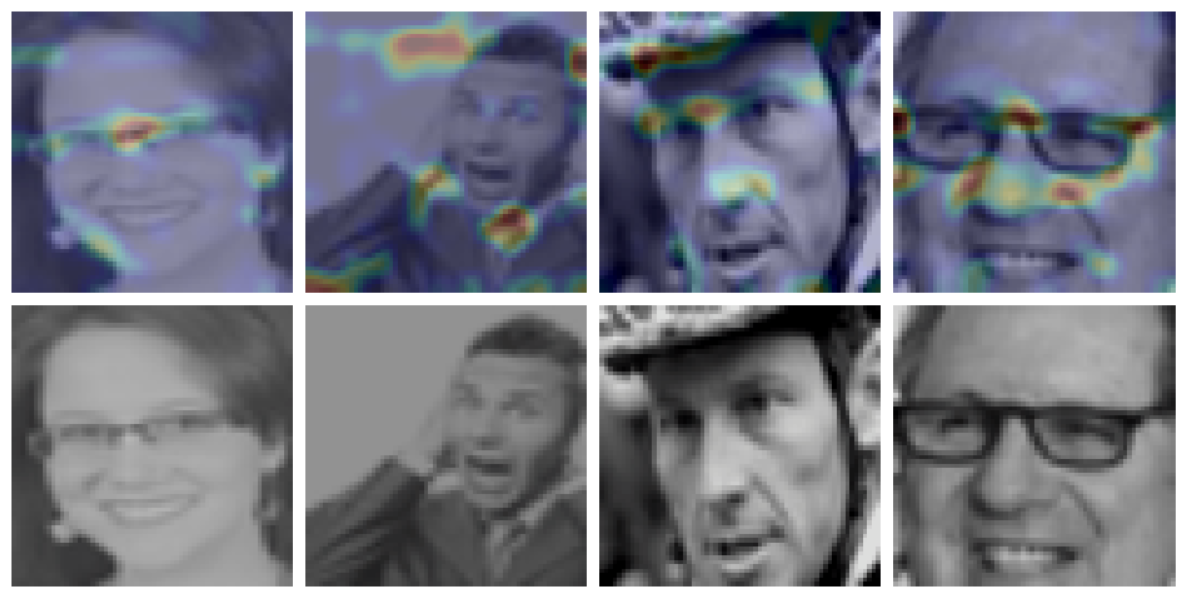
\includegraphics[width=0.8\textwidth]{gradcam_example_faces.png}
    \caption{An example failure case by visualizing the heatmaps of the gradient of a unlabeled SimCLR trained ResNet \citep{chen2020simple} using the GradCAM method \citep{selvaraju2017grad}. The OOD detection task is to detect OOD facial expressions. In this case, the OOD detection method fails as justified by our theoretical work, where the representations do not exhibit a strong gradient in regions commonly associated with facial expressions (i.e., eyebrows, mouth, etc.).}
    \label{fig:grad}
\end{figure}

However, one can unintentionally avoid label blindness problem via the selection of the OOD dataset when constructing OOD benchmarks. Existing methods generally consider ID and OOD data from different datasets, e.g., \citet{fort2021exploring}, \citet{sehwag2021ssd}, and \citet{hendrycks2019using}. In these benchmarks, there is no significant overlap between the ID and OOD input data, allowing OOD detection algorithms to succeed on features independent of the label. To address this issue and to test for label blindness, we introduce the Adjacent OOD detection task to evaluate the performance on OOD detection algorithms when there is significant overlap between the OOD input data and ID input data. We also prove that it is impossible to guarantee that a real world system will never encounter OOD input data that significantly overlaps ID input data.

This work aims to answer the following question: \emph{can we ignore labels when engaging in OOD detection?} Through numerous experiments and theoretical proofs, we show that it is not safe to ignore labels when performing OOD detection. This is contrary to the increasing recent efforts that propose new self supervised, unsupervised, and other unlabeled OOD detection methods. This work's key contributions include:
\begin{itemize}
\item \textbf{The Label Blindness Theorem.} We theoretically prove that any SSL or Unsupervised Learning algorithm will fail when its information required for the surrogate task is independent of the information required for predicting labels. Through this proof, we conclude that there cannot be a generally applicable SSL or Unsupervised learning OOD detection algorithm as there will always exist independent labels due to the no free generalization theorem.

\item \textbf{Adjacent OOD detection benchmarks.} We introduce the concept of bootstrapping without replacement of the ID labels to create the Adjacent OOD detection task. To the authors' knowledge, this OOD detection task is novel to and absent from research in OOD detection. This task evaluates OOD detection when there is significant overlap in OOD data and ID. We also theoretically prove that overlapping OOD and ID data is possible in every real world dataset.

\item \textbf{Impact on existing and future OOD methods.} We demonstrate that existing SSL and Unsupervised Learning OOD methods fail under the conditions suggested by our theory and that existing benchmarks do not capture such failures. We also evaluate zero shot OOD detection methods, which fail in a similar manner to SSL and Unsupervised Learning OOD methods. We make recommendations on the development and testing of future OOD methods.
\end{itemize}

\section{Preliminaries}

\subsection{Labeled and Unlabeled Out-of-Distribution Detection}

The task of out-of-distribution detection is to identify a semantic shift in the data \citep{yang2021generalized}. This is determining when no predicted label could match the true label $\vy \notin \sY_{in}$, where $\sY_{in}$ represents the set of in-distribution training labels. In this case, we would consider the semantic space of the sample and the training distribution to be different, representing a semantic shift. We can express the probability that a sample is out-of-distribution via $P(\vy \notin \sY_{in} | \vx)$. One baseline method to calculate $P(\vy \notin \sY_{in} | \vx)$ is to take $1 - \texttt{MSP}(\vx)$, where $\texttt{MSP}$ is the maximum softmax probability from a classifier for a particular datapoint.

Furthermore, we are only concerned with labels that can be generated using only $\vx$, via function $f$ which depends solely on $\vx$ and no other information. $f$ may represent human labelers that generate $\vy$. If we consider $\sY_{all}$ as the set of all possible labels that can be generated from $f(\vx \in \sX_{all})$, a subset of $\sX_{all}$ considered as $\sX_{training}$ may not contain all labels in $\sY_{all}$. For real world datasets, it is possible that $\sY_{in} \subsetneq \sY_{all}$.

We can also approach the problem of OOD detection without the use of labels. One can train a model on ID data using a surrogate task for the purposes of computing a metric. For example, \citet{sehwag2021ssd} trains a resnet with SimCLR and computes the Mahalanobis distance between the training representations and the test sample representations to compute the OOD score. Alternatively, one could utilize a pretrained model with broad knowledge to compute a metric to use as the OOD score, such as in \citet{wang2023clipn}.

\subsection{Self-Supervised and Unsupervised Learning}

This section covers representation learning and its implications for SSL and unsupervised learning. If there is no mutual information between two random variables, neither can be used to reduce uncertainty about the other \citep{shannon1948mathematical}. In both self-supervised and unsupervised OOD detection, if there is no mutual information between the intermediate representations and the OOD detection task, the OOD detection system cannot reduce uncertainty with respect to the OOD detection task using the intermediate representations.

Representation learning can be formulated as finding a distribution $p(\rvz|\rvx)$ that maps the observations from $\vx \in \sX$ to $\vz \in \sZ$, while capturing relevant information for some primary task. When $\rvy$ represents some primary task, we consider only $\rvz$ that is sufficiently discriminative for accomplishing the task $\rvy$. For simplicity, we consider $\rvy$ as a classification label, but $\rvy$ can represent any objective or task. \citet{federici2020learning} show that this sufficiency is met when the information relevant for predicting $\rvy$ is unchanged when encoding $\rvx \rightarrow \rvz$.

\begin{definition}
    Sufficiency: A representation $\rvz \text { of } \rvx$ is sufficient for $\rvy$ if and only if $I(\rvx ; \rvy \mid \rvz)=0 $.
    \label{definesuff}
\end{definition}

Since there exists the sufficient statistic $\rvx=\rvz$, we must consider the minimal sufficient statistic which conveys only relevant information for predicting $\rvy$. An SSL algorithm seeks to learn the minimal sufficient statistic via the information bottleneck framework \citep{shwartz2023compress}.

\begin{definition}
Minimal Sufficient Statistic. A sufficient statistic $\rvz$ is minimal if, for any other sufficient statistic $\rvs$, there exists a function $f$ such that $\rvz = f(\rvs)$.
\label{defineminsuff}
\end{definition}

Information bottleneck optimization can be expressed as the minimization of the representation's complexity via $I(\rvx;\rvz)$ and maximizing its utility $I(\rvz;\rvy)$. This results in the information theoretic loss function below, where $\beta$ is a trade-off between complexity and utility \citep{shwartz2023compress}. In practice, learning $\rvz$ without $\rvy$ requires a surrogate task $\rvy_{s}$, e.g., \citet{chen2020simple}, with the loss defined as:
\begin{align}
\mathcal{L}=I(\rvx ; \rvz)-\beta I(\rvz ;\rvy).
\end{align}
It should be noted that the primary task $\rvy$ may be equal to the SSL task $\rvy_{s}$. In such a case, compression towards the minimal sufficient statistic still occurs. This is important because unsupervised methods for deep neural networks (DNNs) will use a surrogate task $\rvy_{u}$ to train the DNN's weights. Thus, if we assign the primary task for an unsupervised learning method to be equal to its surrogate task, it will behave identically to SSL from the perspective of information theory.

When $\rvx$ has higher information content than $\rvy$, there exists information in $\rvx$ that is not relevant for predicting $\rvy$. This can be better understood by dividing $I(\rvx;\rvz)$ into two terms \citep{federici2020learning} as follows:
\begin{align}
I(\rvx ; \rvz)=\underbrace{I(\rvx ;\rvz \mid \rvy)}_{\text {superfluous information }}+\underbrace{I(\rvz ; \rvy)}_{\text {predictive information }}. \label{superfluous}
\end{align}

However, superfluous information is not affected by the labels of primary task, only by $\rvx$ and $\rvy_{s}$. Using information theory, we can show that any SSL OOD detection algorithm will fail when the surrogate task $\rvy_{s}$ is independent of the labels in the in-distribution dataset. This applies to unsupervised OOD detection algorithms that also use a surrogate task.

\section{Guaranteed OOD Detection Failure}

This section introduces the concept of \textbf{Label Blindness}, with one key supporting theorem and one key supporting lemma. Note that $R_{\rvx}$ represents the support of random variable $\rvx$ such that $R_{\rvx} = \{\vx \in \R : P(\vx) > 0\}$. For clarity, we refer to cases where $I(\rvx_1; \rvx_2) = 0$ as \textbf{Strict Label Blindness} and discuss \textbf{Approximate Label Blindness} $I(\rvx_1; \rvx_2) \approx 0$ later in this section.

\subsection{Label Blindness Theorem (Strict Label Blindness)}

We identify a guarantee of OOD detection failure for any information bottleneck-based optimization process if the unlabeled learning objective is independent from labels used to determine the ID set, described by Corollary \ref{mainbodyfailood}. This corollary is derived from two concepts: strict label blindness in the minimal sufficient statistic and the independence of filtered distributions. We first consider the minimal sufficient statistic and how it leads to strict label blindness; see Theorem \ref{mainbodygenloss}.

\begin{theorem}[Strict Label Blindness in the Minimal Sufficient Statistic]
    Let $\rvx$ come from a distribution. $\rvx$ is composed of two independent variables $\rvx_1$ and $\rvx_2$. Let $\rvy_1$ be a surrogate task such that $H(\rvy_1|\rvx_1) = 0$. Let $\rvz$ be any sufficient representation of $\rvx$ for $\rvy_1$ that satisfies the sufficiency definition \ref{definesuff} and minimizes the loss function $\mathcal{L} = I(\rvx_1 \rvx_2; \rvz) - \beta I(\rvz;\rvy_1)$. The possible $\rvz$ that minimizes $\mathcal{L}$ and is sufficient must meet the condition $I(\rvx_2; \rvz) = 0$.
    \label{mainbodygenloss}
\end{theorem}

\textit{Proof:} See Appendix \ref{app:genloss} for the complete proof.

Intuitively, the minimal sufficient representation cannot encode any information independent of the surrogate learning objective, otherwise it would not be minimal. This means that the representation will be blind to any label built upon the independent information.

However, Theorem \ref{mainbodygenloss} is not sufficient to guarantee OOD failure. This is because the selection of the ID training set could change the learned representation $\rvz$, possibly improving OOD detection performance by increasing mutual information, $I(\rvx_2;\rvz) > 0$. We formally disprove this possibility through Lemma \ref{mainbodyfilter}.

\begin{lemma}[Independence of Filtered Distributions]
    Let $\rvx$ come from a distribution. $\rvx$ is composed of two independent variables $\rvx_1$ and $\rvx_2$. For $\rvx_2'$ where $R_{\vx_2'} \subset R_{\vx_2}$, there exists no $\rvx_2'$ such that $H(\rvx_1|\rvx_2') < H(\rvx_1)$.
    \label{mainbodyfilter}
\end{lemma}

\textit{Proof:} See Appendix \ref{app:filter} for the complete proof.

Lemma \ref{mainbodyfilter} states that filtering on a label generated on one of two independent variables cannot provide information about the other. This applies to the selection of ID data from the population, if the selection criteria is independent of the learning objective. This means that the strict label blindness properties predicted by Theorem \ref{mainbodygenloss} will apply to ID training data. These two concepts bring us to our main result -- strict label blindness in filtered distributions; see Corollary \ref{mainbodyfailood}.

\begin{corollary}[Strict Label Blindness in Filtered Distributions]
    Let $\rvx$ come from a distribution. $\rvx$ is composed of two independent variables $\rvx_1$ and $\rvx_2$. Let $\rvy_1$ be a surrogate task such generated by $\vy_1 = f_1(\vx_1)$ $H(\rvy_1|\rvx_1) = 0$. Let $\rvy_2$ be a label such that $H(\rvy_2|\rvx_2) = 0$ and $\vy_2 = f_2(\vx_2)$. Let $\sY_{in}$ be as subset of labels $\sY_{in} \subset R_{\rvy_2}$. Let $\rvx'$ be a subset of $\rvx$ where $R_{\rvx'} = R_{\rvx} \cap \{\vx \in \R: f_2(\vx_2) \in \sY_{in} \}$ such that $\rvx'$ is composed of independent variables $\rvx_1'$ and $\rvx_2'$ and $\vy_1' = f_1(\vx_1')$. The sufficient representation $\rvz$ learned by minimizing $\mathcal{L} = I(\rvx_1' \rvx_2'; \rvz) - \beta I(\rvz;\rvy_1')$ must have $I(\rvx_2;\rvz) = 0$ and $I(\rvy_2;\rvz) = 0$.
    \label{mainbodyfailood}
\end{corollary}

\textit{Proof:} See Appendix \ref{app:failood} for the complete proof.

This means that, when we select the ID training data, if the selection criteria and labels are independent of the surrogate learning objective, then we can guarantee failure in OOD detection due to the absence of any information in the learned representation $\rvz$. For simplicity, we refer to this concept, supported by Corollary \ref{mainbodyfailood}, as the problem of \textbf{Strict Label Blindness}.

In summary, when the surrogate learning task can be achieved without learning about features relevant for the label, it will not learn any features relevant for the label. If the SSL or unsupervised learning method fails to learn any label-relevant features, then any OOD detection algorithm built from those representations cannot differentiate between the labels selected as ID and those not selected as ID. This guarantees failure in OOD detection because no label information passes through the information bottleneck.

\subsection{Implications of Strict Label Blindness in Real World Situations}

We can utilize Fano Inequality to extend our understanding of strict label blindness to consider situations where the variables are not fully independent. The lower bound for prediction error is defined by the entropy of the target label $\rvy$ less the mutual information between the input $\rvx$ and target label, as shown in Theorem \ref{fano}. Under strict label blindness, when $I(\rvx;\rvy) = 0$, the lower bound for error is at its maximum. When $I(\rvx;\rvy) \approx 0$, the lower bound for error is large enough to be unreliable. We refer to this condition as \textbf{Approximate Label Blindness} and we conduct experiments to evaluate this condition. Unless specified as strict, label blindness refers to the approximate case.

\begin{theorem}[Fano's Inequality]
Let $\rvy$ be a discrete random variable representing the true label with $\mathcal{Y}$ possible values and cardinality of $|\mathcal{Y}|$ and $\rvx$ be a random variable used to predict $\rvy$. Let $e$ be the occurrence of an error such that $\rvy \neq \hat{\rvy}$ where $\hat{\rvy} = f(\rvx)$. Let $H_b$ represent the binary entropy function such that $H_b(e)=-P(e) \log P(e)-(1-P(e)) \log (1-P(e))$. The lower bound for $P(e)$ increases with lower $I(\rvx;\rvy)$.
\begin{align}
H_b(e) + P(e) \log(| \mathcal{Y} |-1) \geq H(\rvy) - I(\rvx; \rvy).
\end{align}
\label{fano}
\end{theorem}

\subsection{Theoretical Implications}

Our work applies to deep neural networks (DNNs) trained without labels for the purpose of OOD detection. The key assumption of information bottleneck compression is generally applicable to DNNs \citep{shwartz2017opening}. Regardless of other assumptions, such as the multi-view assumption, an information bottleneck DNN trained without labels will still compress data irrelevant to its loss objective, even if that data is relevant for its intended task. It does not matter what task the training process was originally designed for because the unlabeled training process ultimately generates/adheres to its own learning objective. For any learning objective, there will exist an independent feature unless compression is not possible, as in $I(\rvx;\rvy) = I(\rvx;\rvx)$. If there is compression, then there exists labels for which OOD detection failure is guaranteed.

Our work predicts a guarantee of failure only when we consider the OOD set of all non-ID data. In our own experiments and in work by \citet{sehwag2021ssd, hendrycks2019using, liu2023unsupervised}, purely self-supervised and unsupervised OOD methods can perform well against common benchmark OOD sets. This suggests that the choice of ID set and OOD set pairs can unintentionally hide label blindness failure. Alternatively, we can also construct a test to identify if the OOD detection algorithm suffers from label blindness. To construct such a test, we rely on the insight from Corollary \ref{mainbodyfailood} and the use of a simple statistical method.

\section{Benchmarking for Label Blindness Failure}

\subsection{Bootstrapping and the Adjacent OOD Benchmark}

One logical consequence of Corollary \ref{mainbodyfailood} is that one cannot avoid failure due to label blindness by selecting different labels for one's ID set, so long as the label selection is independent from the learning objective. To test any OOD detection algorithm for label blindness failure, this simply entails selecting different labels for one's ID set. To construct this benchmark, we randomly sample labels to be considered as ID and other labels to be consider OOD. This is similar to bootstrapping, but without replacement. If an OOD detection algorithm is `approximately label blind', its average OOD detection performance across the samples should be poor. We refer to this as the \textbf{Adjacent OOD Detection Benchmark}.

\subsection{Why Adjacent OOD is Safety-Critical to Almost All Real World Systems}

The Adjacent OOD detection benchmark evaluates the performance of OOD detection algorithms when there may be a significant overlap between the ID data and OOD data. This condition applies to all systems where it is impossible to guarantee that there will be no significant overlap in the feature space between ID and OOD data. This is true for almost all real world systems and is theoretically proven below.

\begin{theorem}[Unavoidable Risk of Overlapping OOD Data]
Let $\rvx$ come from a distribution. Let $f$ be some labeling function to generate labels $\rvy$ such that $\vy = f(\vx)$, where there are at least two unique labels $|R_\rvy| > 1$. Let $\rvx_{in}$ be a random subset of $\rvx$ where $R_{\rvx_{in}} \subsetneq R_\rvx$ and $|R_{\rvx_{in}}| < \infty$. Let $\rvy_{in}$ be labels generated from $\vy_{in} = f(\vx_{in})$. The probability that a randomly selected $\vx$ contains $\vy$ not present in $R_{\rvy_{in}}$ is always greater than 0.
\label{mainbodyoverlap}
\end{theorem}

\textit{Proof:} See Appendix \ref{app:overlaprisk} for the complete proof.

In theory, this risk can be reduced to an acceptable level by adding more data to the training dataset. However, this reduction in risk requires the assumption that the collected data is randomly sampled. This is almost never true for real world datasets and often the opposite is true, where the nature of sampling can significantly increase this risk.

One risk factor present in every real world dataset is the dataset creation date. By creating the dataset at any specific point in time, the dataset cannot be randomly sampled with respect to time because it is impossible to collect data from the future. For example, if one were to create a dataset of diseases today, it would not contain any future diseases. In this example, the probability that the training dataset is incomplete is 100\%, which guarantees that there will be OOD data that significantly overlaps with ID data. For most real world systems, the only safe assumption is that there may be OOD data that overlaps with ID data and it is necessary to plan accordingly.

The failure predicted by the label blindness theory is easiest to detect in the adjacent OOD situation. Where there is a likelihood of adjacent data, Theorem \ref{mainbodyfailood} predicts OOD detection failure. Where there is no adjacent data, features independent of the label can still be used to distinguish between ID data and non adjacent OOD data, as shown in various experiments in this paper and others \citep{sehwag2021ssd, hendrycks2019using, liu2023unsupervised}.

\subsection{Comparing Adjacent, Near, and Far OOD Benchmarks}

Many unlabeled OOD methods generally perform quite well on far and near OOD tasks. Far OOD is often defined by ID and OOD sets with different semantic labels and styles \citep{fang2022out}. One such far OOD benchmark is MNIST as ID data and CIFAR10 as OOD data. Near OOD contains ID and OOD sets with similar semantic labels and styles \citep{fang2022out}. These tasks tend to be more difficult for existing OOD detection methods than far OOD detection tasks. One such near OOD benchmark is CIFAR10 as ID and CIFAR100 as OOD. However, the overlap in the near OOD detection benchmarks is significantly less than the adjacent OOD detection benchmark, which evaluates the maximum possible feature overlap. For example, an Adjacent OOD benchmark on the ICML Facial Expressions dataset may contain the same face with different expressions, resulting in significant feature overlap. These existing benchmarks do not provide sufficient safety guarantees in applications where there may be significant overlap between ID and OOD data.

\subsection{Implications for OOD from Unlabeled Data}

While methods that utilize only unlabeled data, such as \citet{sehwag2021ssd, liu2023unsupervised, guille2024cadet}, show promising results on both near and far OOD tasks, their performance in the adjacent OOD detection tasks depends on the mutual information between the learned representation and the ID labels. Our theoretical work suggests that such methods will perform poorly, if the surrogate task is independent of the labels.

The adjacent OOD detection benchmark can also evaluate the performance of zero shot OOD detection methods. While our theoretical work does not extend to pretraining due to the use of labels, it is also still important to consider the performance when OOD data overlaps ID data.

\section{Experimental Results}

We conduct the following experiments to verify the existence of label blindness in unlabeled OOD detection methods. All hyperparameters and configurations were the best performing from their respective original paper implementations, unless noted otherwise. Experiments are repeated 3 times.

\subsection{Experimental Setup}

\paragraph{Supervised Baseline.}
We use Maximum Softmax Probability (MSP) \citep{hendrycks2016baseline} as our baseline supervised method for comparison. We augment the training data using random rotation, horizontal flip, random crop, gray scale, and color jitter. Images are resized to $64\times64$. We train using stochastic gradient descent with momentum and a cosine annealing learning schedule. We train for $10$ warm up epochs followed by $150$ regular epochs, selecting the weights with the highest validation accuracy. We use a standard ResNet50 architecture.

\paragraph{Self-supervised Baselines.}
We use two SSL methods to evaluate how representations are learned, SimCLR \citep{chen2020simple} and Rotation Loss (RotLoss) \citep{hendrycks2019using}. Images are resized to $64\times64$ for both cases. For SimCLR, we augment the training data using random rotation, horizontal flip, random crop, gray scale, and color jitter. For Rotation Loss, we use only random crop and horizontal flip. We train using stochastic gradient descent with momentum (and a cosine annealing learning schedule) and employ a standard ResNet50 architecture and train for $10$ warm up epochs followed by $500$ regular epochs, selecting the weights with the best-learned representations. We use a KNN classifier to determine the best representations during validation at the end of each epoch.

To evaluate OOD performance, we use two methods to generate the OOD score of each sample, SSD \citep{sehwag2021ssd} and KNN, similar to \citet{sun2022out}. SSD considers the OOD score as the Mahalanobis distance of the sample from the center of all in-distribution training data samples. The KNN method considers the OOD score as the Euclidean distance from the $N$th nearest neighbor of the test sample to all in-distribution training samples. Both methods are distance based OOD detection and are commonly used with representation learning. We use the same representation mentioned in the previous paragraph.

\paragraph{Unsupervised Baseline.}
To consider how an unsupervised OOD detection method functions, we evaluate the diffusion impainting OOD detection method proposed by \citet{liu2023unsupervised} using code provided in their paper's linked repository. We utilize the training configuration that generated the paper's main results, which involved an alternating checkerboard mask 8 × 8, an LPIPS distance metric to calculate the OOD score, and 10 reconstructions per image. We modify only the input image size to be $64\times64$ for all datasets and run additional experiments to evaluate performance on their alternative MSE distance metric. This method is representative of other generative methods, such as \citet{xiao2020likelihood}.

\paragraph{Zero-shot Baseline.}
To consider how well zero shot learning algorithms perform, we evaluate the CLIPN model presented by \citet{wang2023clipn}. We utilize their pretrained weights provided in their paper's repository and perform zero shot OOD detection on our adjacent OOD detection benchmark. We evaluate CLIPNs performance using 3 of their paper's algorithms, Maximum Softmax Probability, Compete to Win (CTW), and Agree to Differ (ATD).

\subsection{Adjacent OOD Datasets}

To create the Adjacent OOD detection task, we randomly split $25$\% of all classes into the OOD set and retain $75$\% as the ID set. We also repeat our experiments three times with different seeds to account for different splits of the ID and OOD set. Only ICML Facial expressions has a major class imbalance for one of its seven classes.

The ICML Facial Expressions dataset \citep{icmlface} contains seven facial expressions split across $28,709$ faces in the train set and $7,178$ in the test set. The expressions include anger, disgust, fear, happiness, sadness, surprise, and neutral. Self-supervised algorithms may not learn relevant features for distinguishing expressions and instead learn features relevant for distinguishing faces.

The Stanford Cars dataset \citep{KrauseStarkDengFei-Fei_3DRR2013} contains $16,185$ images taken from $196$ classes of cars. The data is split into $8,144$ training images and $8,041$ testing images, with each class being split roughly $50$-$50$. Classes are typically very fine-grained, at the level of Make, Model, Year, e.g., 2012 Tesla Model S or 2012 BMW M3 coupe. This creates a particularly challenging Adjacent OOD task because of the reliance on more subtle features to differentiate cars.

The Food 101 dataset by \citet{bossard14} consists of $101$ food categories and $101,000$ images. There are $250$ manually reviewed test images and $750$ training images for each class. Note that training images were not cleaned to the same standard as the test images and will contain some mislabeled samples. We believe that this should not significantly detract from the Adjacent OOD nature of the dataset.

\subsection{Experimental Results}

Experimental results for Adjacent OOD are presented in Table \ref{tab:results}. It is apparent that the baseline supervised method performs better than most unlabeled methods on the Adjacent OOD detection task. In cases where the unlabeled methods exhibits performance as good as random guessing, it is likely that the learned representation contains little information about the semantic label. This is contrary to the reported performance improvements presented in unlabeled OOD papers \citep{sehwag2021ssd, hendrycks2019using, liu2023unsupervised}, as our experimental results suggest unlabeled OOD is significantly worse than a simple MSP baseline.

It is important to note that the zero shot CLIPN method performs well when the label text's usage in pretraining is similar to the label text's usage in the ID data. In the case of the Cars dataset, the pretraining dataset CC3M \citep{sharma2018conceptual} contains many images captioned with the make and model of various cars, resulting in good performance. The Food dataset also sees similar label usage in the pretraining set. However, the Faces dataset's labels are not aligned. For example, there are multiple images associated with the emotion angry that do not contain a human face, such as an image of a angry fist. When there is little or no mutual information between the pretraining data and the ID labels, zero shot methods will perform poorly in OOD detection tasks.

\begin{table}[h]
\caption{Results from experiments across various datasets and methods. Unlabeled methods perform poorly in adjacent OOD detection. CLIPN performance is due to labels present in the pretraining dataset. Higher AUROC and lower FPR is better.}
\vspace{2mm}
\centering
\begin{tabular}{l|ll|ll|ll}
\toprule
                & Faces    &          & Cars     &           & Food     &          \\ \hline
Method          & AUROC    & FPR95    & AUROC    & FPR95     & AUROC    & FPR95    \\ \midrule
Supervised MSP  & 70.8±0.3 & 88.2±0.2 & 69.2±0.9 & 88.8±0.8  & 78.8±1.2 & 81.1±1.6 \\ \midrule
SimCLR KNN      & 52.0±4.2 & 95.0±1.3 & 52.5±0.4 & 94.0±0.5  & 61.1±2.8 & 91.6±1.6 \\
SimCLR SSD      & 55.0±4.5 & 95.1±2.0 & 52.7±0.7 & 93.7±1.1  & 64.4±0.8 & 89.3±0.5 \\
RotLoss KNN     & 46.1±2.5 & 95.8±0.4 & 51.1±0.6 & 94.8±0.7  & 49.7±3.8 & 94.9±0.9 \\
RotLoss SSD     & 46.6±3.0 & 95.7±0.5 & 50.7±1.9 & 95.0±1.2  & 50.7±3.6 & 94.9±0.9 \\ \midrule
Diffusion LPIPS & 54.7±4.6 & 94.2±3.7 & 53.8±1.8 & 93.9±1.2  & 52.9±2.2 & 94.4±0.6 \\
Diffusion MSE   & 55.3±2.2 & 94.2±1.4 & 51.6±1.6 & 94.4±0.5  & 52.5±3.4 & 94.2±0.6 \\ \midrule
CLIPN CTW       & 47.0±1.4   & 97.3±0.3 & 65.0±5.1   & 69.4±9.4  & 70.9±2.9 & 69.1±7.0   \\
CLIPN ATD       & 44.2±1.4 & 97.5±0.2 & 81.1±4.3 & 56.6±10.4 & 84.9±0.2 & 53.9±4.5 \\
CLIPN MSP       & 58.7±4.4 & 95.9±1.4 & 76.5±1.4 & 75.4±0.6  & 80.5±1.6 & 74.0±1.4   \\ \bottomrule
\end{tabular}
\label{tab:results}
\end{table}

We observe decent OOD performance on the unlabeled SimCLR compared to the labeled supervised MSP for CIFAR10 and CIFAR100 datasets. This is likely because the SimCLR algorithm is better at learning the relevant features in these datasets and that the classes are more visually dissimilar, resulting in less overlap of OOD and ID data. We also show strong results for far OOD performance for SimCLR based OOD detection, which confirms findings in papers that test unlabeled OOD methods against a far OOD detection benchmark \citep{sehwag2021ssd, tack2020csi, liu2023unsupervised, guille2024cadet, wang2023clipn}.

\section{Discussion}

\subsection{Impact of Label Blindness on Future Research}

A consequence of the label blindness theorem is that there cannot exist a single unlabeled OOD detection algorithm for all unlabeled data. However, unlabeled learning methods, such as SimCLR, are vital for improving OOD detection. The model of \citet{sun2022out} learns representations using a supervised version of SimCLR, similar to \citet{khosla2020supervised}. The combination of a multi-view information bottleneck with supervised classes produces a more robust representation of the in-distribution data than using only a supervised loss. Recent work by \citet{du2024does} provides a strong theoretical basis for why unlabeled data can improve OOD detection performance.

The Adjacent OOD detection benchmark addresses a critical safety gap in existing OOD detection research. Current benchmarks often use datasets with minimal feature overlap between ID and OOD data, which can mask the label blindness problem. In real-world applications, especially safety-critical ones, it is essential to evaluate OOD detection methods under conditions where ID and OOD data may have significant feature overlap.

Our findings suggest that practitioners should be cautious when deploying unlabeled OOD detection methods in scenarios where the training data may not capture all relevant semantic variations. The theoretical guarantees provided by our label blindness analysis indicate that such methods may fail catastrophically when encountering OOD data that shares features with ID data but differs in the semantic labels.

\subsection{Recommendations for Future OOD Detection Research}

Based on our theoretical and empirical findings, we recommend several directions for future research:

\begin{itemize}
\item \textbf{Hybrid approaches}: Combining supervised and self-supervised learning objectives may help mitigate label blindness by ensuring that label-relevant features are preserved during representation learning.

\item \textbf{Adjacent OOD evaluation}: All OOD detection methods should be evaluated on Adjacent OOD benchmarks to assess their robustness to scenarios with high feature overlap between ID and OOD data.

\item \textbf{Information-theoretic analysis}: Future unlabeled OOD detection methods should include theoretical analysis of the mutual information between their learning objectives and the target labels to identify potential label blindness issues.

\item \textbf{Domain-aware methods}: Developing methods that can explicitly model and account for domain-specific features may help address some of the limitations identified in our work.
\end{itemize}

\section{Conclusion}

In this work we provide an answer to the question, can we ignore labels for OOD detection? Our theoretical work shows that the answer is no, unless the unlabeled method happens to capture the relevant features and does not need to work for different sets of labels. Due to the lack of existing benchmarks that capture the theoretically expected failure, we introduce a novel type of OOD task, Adjacent OOD detection. This task addresses the critical safety gap caused by significant overlap of ID and OOD data. We show that the Adjacent OOD task accurately captures the failure in unlabeled OOD detection that is hypothesized by our theory.

The label blindness theorem demonstrates that when the surrogate learning task used in self-supervised or unsupervised learning is independent of the features relevant for label prediction, OOD detection is guaranteed to fail. This fundamental limitation cannot be overcome by simply selecting different ID datasets, as the independence property is preserved under filtering operations.

Our experimental results confirm the theoretical predictions, showing that unlabeled OOD detection methods perform poorly on Adjacent OOD benchmarks where there is significant feature overlap between ID and OOD data. In contrast, these same methods often perform well on traditional far OOD benchmarks, highlighting the importance of comprehensive evaluation.

The Adjacent OOD detection benchmark introduced in this work provides a crucial tool for evaluating the robustness of OOD detection methods in realistic scenarios. This benchmark addresses a previously ignored safety gap in OOD detection research and should be adopted as a standard evaluation protocol for future work.

We hope our work will help support more robust research into OOD detection and improve the safety of AI applications. The theoretical framework and empirical findings presented here provide important guidance for developing more reliable OOD detection methods that can handle the complexities of real-world deployment scenarios.





\chapter{Domain Feature Collapse: How Single Domain Training Removes Domain Features}

This chapter covers on going research. 


\chapter{Are Hallucinations Out of Distribution?}

This chapter covers a proposal to research the nature of hallucinations. 

\chapter{Research Timeline}

\chapter{Discussion}



% Bibliography (using BibTeX database (.bib))
\bibliographystyle{iclr2025_conference}
\bibliography{Bibliography}

% (OPTIONAL) Appendices
\begin{appendices}
\chapter{Theoretical Proofs for Label Blindness}
\label{app:proofs}

This appendix contains the detailed theoretical proofs supporting the Label Blindness theory presented in Chapter 4. The proofs establish the mathematical foundations for understanding when and why unlabeled out-of-distribution detection methods are guaranteed to fail.

\section{Properties of Mutual Information and Entropy}
\label{app:properties}

In this section we enumerate some of the properties of mutual information that are used to prove the theorems reported in this work. For any random variables $\rvw, \rvx, \rvy$ and $\rvz$:

$\left(P_1\right)$ Positivity:
$$
I(\rvx ; \rvy) \geq 0, I(\rvx ; \rvy \mid \rvz) \geq 0
$$
$\left(P_2\right)$ Chain rule:
$$
I(\rvx \rvy ; \rvz)=I(\rvy ; \rvz)+I(\rvx ; \rvz \mid \rvy)
$$
$\left(P_3\right)$ Chain rule (Multivariate Mutual Information):
$$
I(\rvx ; \rvy ; \rvz)=I(\rvy ; \rvz)-I(\rvy ; \rvz \mid \rvx)
$$
$\left(P_4\right)$ Positivity of discrete entropy:
For discrete $\rvx$
$$
H(\rvx) \geq 0, H(\rvx \mid \rvy) \geq 0
$$
$\left(P_5\right)$ Entropy and Mutual Information
$$
H(\rvx)=H(\rvx \mid \rvy)+I(\rvx ; \rvy)
$$

$(P_6)$ Conditioning a variable cannot increase its entropy

$$
H(\rvy|\rvz) \leq H(\rvy)
$$

$(P_7)$ A variable knows about itself as much as any other variable can

$$
I(\rvx;\rvx) \geq I(\rvx;\rvy)
$$

$(P_8)$ Symmetry of Mutual Information

$$
I(\rvx;\rvy) = I(\rvy;\rvx)
$$

$(P_9)$ Entropy and Conditional Mutual Information (This is simply $P_5$ conditioned on $\rvz$)

$$
I(\rvx;\rvy|\rvz)  = H(\rvx|\rvz) - H(\rvx|\rvy\rvz)
$$

$(P_{10})$ Functions of Independent Variables Remain Independent

$$
I(\rvx; \rvy) = 0 \rightarrow I(f(\rvx);\rvy) = 0
$$

\section{Supporting Theorems and Proofs}
\label{app:supporting}

This section contains supporting theorems and proofs that establish the foundation for the main Label Blindness results.

\subsection{Sufficiency}
\label{app:sufficiency}

\begin{proposition}
Let $\rvx$ and $\rvy$ be random variables from joint distribution $p(\rvx, \rvy)$. Let $\rvz$ be a representation of $\rvx$, then $\rvz$ is sufficient for $\rvy$ if and only if $I(\rvx ; \rvy)=I(\rvy ; \rvz)$

Hypothesis:

$\left(H_1\right) \rvz$ is a representation of $\rvx: I(\rvy ; \rvz \mid \rvx)=0$

Thesis:

$\left(T_1\right) I(\rvx ; \rvy \mid \rvz)=0 \Longleftrightarrow I(\rvx ; \rvy)=I(\rvy ; \rvz)$

\begin{proof}
$$
\begin{aligned}
I(\rvx ; \rvy \mid \rvz) & \stackrel{\left(P_3\right)}{=} I(\rvx ; \rvy)-I(\rvx ; \rvy ; \rvz) \stackrel{\left(P_3\right)}{=} I(\rvx ; \rvy)-I(\rvy ; \rvz)+I(\rvy ; \rvz \mid \rvx) \\
& \stackrel{\left(H_1\right)}{=} I(\rvx ; \rvy)-I(\rvy ; \rvz)
\end{aligned}
$$

Since both $I(\rvx ; \rvy)$ and $I(\rvy ; \rvz)$ are non-negative $\left(P_1\right), I(\rvx ; \rvy \mid \rvz)=0 \Longleftrightarrow I(\rvy ; \rvz)=I(\rvx ; \rvy)$

\end{proof}
\label{sufficiency}
\end{proposition}

\subsection{Lower Bound of Mutual Information for Sufficiency}
\label{app:infobound}

\begin{lemma}
Let $\rvx$ and $\rvy$ be random variables with joint distribution $p(\rvx, \rvy)$. Let $\rvz$ be a representation of $\rvx$ that is sufficient, as per definition \ref{definesuff}. Then $I(\rvx;\rvz) \geq I(\rvz;\rvy)$ and $I(\rvx;\rvz) \geq I(\rvx;\rvy)$.

Hypothesis:

$(H_1)$ $\rvz$ is a representation of $\rvx: I(\rvy ; \rvz \mid \rvx)=0$

$(H_2)$ $ \rvz$ is a sufficient representation of $\rvx: I(\rvx; \rvy| \rvz))=0$

Thesis:

$(T_1)$ $\forall \rvz.I(\rvx;\rvz) \geq I(\rvz;\rvy), I(\rvx;\rvz) \geq I(\rvx;\rvy)$

\begin{proof}By Construction

$$
\begin{aligned}
I(\rvx \rvy|\rvz)) &\stackrel{\left(H_2\right)}{=} 0 \\
&\stackrel{\left(P_2\right)}{=} I(\rvz \rvy; \rvx) - I(\rvz; \rvx) \\
&\stackrel{\left(P_2\right)}{=} I(\rvx; \rvy) + I(\rvx; \rvz|\rvy) - I(\rvz; \rvx) \\
&\stackrel{\left(PropB1\right)}{=} I(\rvz; \rvy) + I(\rvx; \rvz|\rvy) - I(\rvz;\rvx) \\
I(\rvz;\rvx) &= I(\rvz;\rvy) + I(\rvx; \rvz|\rvy)\\
I(\rvz;\rvx) &\stackrel{\left(P_1\right)}{\geq} I(\rvz; \rvy)\\
\end{aligned}
$$

Note that $I(\rvz; \rvy) = I(\rvx; \rvy)$ for all sufficient representations, as per proposition \ref{sufficiency}.

This supports our intuition that the information in the representation consists of relevant information $I(\rvz;\rvy)$ and irrelevant information $I(\rvx; \rvz| \rvy)$. By definition of sufficiency, there must be enough information for $I(\rvz; \rvy)$ in $I(\rvx; \rvz)$, which is to say that the size of the encoding cannot be smaller than the minimum size to encode all of $I(\rvx; \rvy)$.

\end{proof}
\label{infobound}
\end{lemma}

\subsection{Conditional Mutual Information of Noise}
\label{app:infonoise}

\begin{lemma}
Let $\rvx$ and $\rvy$ be independent random variables and $\rvz$ be a function of $\rvx$ with joint distribution $p(\rvx, \rvy, \rvz)$. The conditional mutual information $I(\rvx; \rvz| \rvy)$ is always equal to the mutual information $I(\rvx; \rvz)$. As in the information content is unchanged when adding noise.

Hypothesis:

$(H_1)$ Independence of $\rvx$ and $\rvy$ : $I(\rvx;\rvy) = 0$

$(H_2)$  $\rvz$ is fully determined by $\rvx$ : $H(\rvz|\rvx) = 0$

Thesis:

$(T_1)$ $I(\rvx; \rvz| \rvy) = I(\rvx; \rvz)$

\begin{proof}
By Construction.

$(C_1)$ Demonstrates that $H(\rvz| \rvx \rvy) = 0$

$$
\begin{aligned}
0 \stackrel{\left(P_4\right)}{\leq} H(\rvz|\rvx \rvy)&\stackrel{\left(P_6\right)}{\leq}H(\rvz|\rvx)\\
H(\rvz|\rvx \rvy)&\stackrel{\left(H_2\right)}{\leq} 0
\end{aligned}
$$

$(C_2)$ Demonstrates that $I(\rvz;\rvy) = 0$
$$
\begin{aligned}
I(\rvz; \rvy)&\stackrel{\left(H_2\right)}{=}I(f(\rvx);\rvy)\\
&\stackrel{\left(P_{10}\right)}{=}I(\rvx ; \rvy)\\
&\stackrel{\left(H_{1}\right)}{=}0\\
\end{aligned}
$$

Thus

$$
\begin{aligned}
I(\rvx; \rvz| \rvy) &\stackrel{\left(P_9\right)}{=} H(\rvz|\rvy) - H(\rvz|\rvx \rvy)\\
&\stackrel{\left(C_1\right)}{=} H(\rvz| \rvy)- 0\\
&\stackrel{\left(P_5\right)}{=} H(\rvz) - I(\rvz; \rvy) \\
&\stackrel{\left(C_2\right)}{=}H(\rvz) - 0 \\
&\stackrel{\left(H_2\right)}{=}H(\rvz) - H(\rvz| \rvx) \\
&\stackrel{\left(P_5\right)}{=}I(\rvx; \rvz)
\end{aligned}
$$

This supports the intuition that if one added a random noise channel it will not change the mutual information.

\end{proof}
\label{infonoise}
\end{lemma}

\subsection{Factorization of Bottleneck Loss}
\label{app:lossfact}

\begin{lemma}
Let $\rvx$ be a random variable with label $\rvy$ such that $H(\rvy| \rvx) = 0$ and $\rvz$ is a sufficient representation of $\rvx$ for $\rvy$. The loss function
$\mathcal{L}=I(\rvx; \rvz)-\beta I(\rvz; \rvy)$ is equivalent to $\mathcal{L}=H(\rvz)-\beta I(\rvz; \rvy)$, with $\beta$ as some constant.

Hypothesis:

$(H_1)$  $\rvz$ is fully determined by $\rvx$ : $H(\rvz|\rvx) = 0$

Thesis:

$(T_1)$ $ I(\rvx; \rvz)-\beta I(\rvz; \rvy) = H(\rvz)-\beta I(\rvz; \rvy)$

\begin{proof} By Construction.
$$
\begin{aligned}
I(\rvx; \rvz)-\beta I(\rvz; \rvy) &\stackrel{\left(P_5\right)}{=} H(\rvz) - H(\rvz| \rvx) -\beta I(\rvz;\rvy) \\
&\stackrel{\left(H_1\right)}{=} H(\rvz) -\beta I(\rvz; \rvy)
\end{aligned}
$$

Due to the relationship between $\rvx$ and $\rvz$, we can create an intuitive factorization of the bottleneck loss function. Effectively, we want to maximize $I(\rvz; \rvy)$ while minimizing the information content of $\rvz$

\end{proof}

\label{lossfact}
\end{lemma}

\section{Main Theorems and Proofs}
\label{app:mainproofs}

We ignore cases where the determined variable has an entropy of 0. Generally, if $H(\rvy| \rvx) = 0 \rightarrow H(\rvy) > 0$. Also, we only consider cases where the random variables have more than zero entropy.

Note that $R_{\rvx}$ represents the support of random variable $\rvx$ such that $R_{\rvx} = \{\vx \in \R : P(\vx) > 0\}$.

\subsection{Strict Label Blindness in the Minimal Sufficient Statistic}
\label{app:genloss}

\begin{theorem}[Strict Label Blindness in the Minimal Sufficient Statistic]
Let $\rvx$ come from a distribution. $\rvx$ is composed of two independent variables $\rvx_1$ and $\rvx_2$. Let $\rvy_1$ be a surrogate task such that $H(\rvy_1|\rvx_1) = 0$. Let $\rvz$ be any sufficient representation of $\rvx$ for $\rvy_1$ that satisfies the sufficiency definition \ref{definesuff} and minimizes the loss function $\mathcal{L} = I(\rvx_1 \rvx_2; \rvz) - \beta I(\rvz;\rvy_1)$. The possible $\rvz$ that minimizes $\mathcal{L}$  and is sufficient must meet the condition $I(\rvx_2; \rvz) = 0$.

\textbf{Summary:} This proof uses the derivative of the loss function to establish the possible set of local minima that satisfies $\mathcal{L}$. For any possible minima of $\mathcal{L}$, the representation $\rvz$ must contain information of only  $\rvx_1 \rightarrow H(\rvz|\rvx_1)=0$ or only $\rvx_2 \rightarrow H(\rvz| \rvx_2)=0)$ or both $\rvx_1, \rvx_2 \rightarrow H(\rvz|\rvx_1, \rvx_2)=0$. We show that   possible set of all local minima must satisfy $H(\rvz|\rvx_1)=0$ by showing that the other two cases must always have greater $\mathcal{L}$. This proves the Theorem that the learned representation cannot contain information about $\rvx_2$.

Hypothesis:

$(H_1)$  $\rvz$ is fully determined by $\rvx$ : $H(\rvz|\rvx) = 0$

$(H_2)$  $\rvz$ is a representation of $\rvx: I(\rvy ; \rvz \mid \rvx)=0$

$(H_3)$  $\rvz$ is a sufficient representation of $\rvx: I(\rvx ; \rvy | \rvz)=0$

$(H_4)$ $\rvx$ is composed of two independent variables $\rvx_1, \rvx_2$ : $\rvx = \rvx_1, \rvx_2, I(\rvx_1; \rvx_2) = 0$

$(H_5)$ $\rvy$ is fully determined by $\rvx_1$: $H(\rvy| \rvx_1) = 0$

Thesis:

$(T_1)$ $\forall \rvz.I(\rvx_2,\rvz) = 0$

\begin{proof} By Construction

$(C_1)$ demonstrates that $\mathcal{L}=H(\rvz) -\beta I(\rvz;\rvy)$ via factoring $I(\rvx_1 \rvx_2;\rvz)$. Alternatively, Theorem \ref{lossfact} creates the same result.

$$
\begin{aligned}
I(\rvx_1, \rvx_2; \rvz) &\stackrel{\left(P_2\right)}{=} I(\rvx_1; \rvz) + I(\rvx_2; \rvz| \rvx_1)\\
&\stackrel{\left(P_5\right)}{=} H(\rvz) -  H(\rvz| \rvx_1) + I(\rvx_2; \rvz| \rvx_1) \\
&\stackrel{\left(P_9\right)}{=} H(\rvz) -  H(\rvz| \rvx_1) + H(\rvz| \rvx_1) - H(\rvz| \rvx_1 \rvx_2) \\
&\stackrel{\left(H_1\right)}{=}H(\rvz) -  H(\rvz| \rvx_1) + H(\rvz| \rvx_1) - 0 \\
&\mathcal{L}=H(\rvz)  -\beta I(\rvz; \rvy)
\end{aligned}
$$

$(C_2)$ Demonstrates that $I(\rvz; \rvy) = I(\rvx; \rvy)$ as per Theorem \ref{sufficiency}.

$(C_3)$ Demonstrates that $I(\rvz; \rvy)$ is a constant across all sufficient representations because Theorem \ref{sufficiency} applies.

$(C_4)$ Demonstrates that for all possible $\rvz$ satisfying $(H_3)$, their loss can be compared using only $\mathcal{L}_z = H(\rvz)$ for comparing across $\rvz$

$$
\begin{aligned}
\frac{d\mathcal{L}}{d\rvz}  &\stackrel{\left(C_1\right)}{=}\frac{H(\rvz)}{d\rvz} - \frac{\beta I(\rvz; \rvy)}{d\rvz} \\
&\stackrel{\left(C_3\right)}{=}\frac{H(\rvz)}{d\rvz} - 0
\end{aligned}
$$

$(C_5)$ Demonstrates that the value of $H(\rvz)$ at all possible $\rvz$ that minimizes $\mathcal{L}$ is the same. Even for different minimal $\rvz$, they must have the same $H(\rvz)$ to all be minimal. When comparing possible minimal solutions to $\mathcal{L}$, $H(\rvz)$ is constant across all minimal solutions.

$(C_6)$ Demonstrates that any $\rvz$ that satisfies sufficiency must satisfy $I(\rvz; \rvx) \geq I(\rvz; \rvy)$ and $I(\rvz; \rvx) \geq I(\rvx; \rvy)$ as per Theorem \ref{infobound}.

$(C_7)$ Demonstrates that minima(s) exists only where $H(\rvz) = I(\rvz; \rvy)$ and $H(\rvz| \rvx) = 0$. Note that $H(\rvz) = I(\rvx; \rvy) = I(\rvz; \rvy)$ is the most compact representation size that is sufficient.

$$
\begin{aligned}
I(\rvz;\rvx) &\stackrel{\left(C_6\right)}{\geq} I(\rvz; \rvy) \\
H(\rvz) - H(\rvz| \rvx)  &\stackrel{\left(P_5\right)}{\geq} I(\rvz; \rvy)\\
\forall \rvz | C_6 \land H_3 \land I(\rvz; \rvx) > I(\rvz; \rvy) &. \exists \rvz'|\rvz' = f(\rvz) \land I(\rvz; \rvx) > I(\rvz'; \rvx) \land C_6 \land H_3
\end{aligned}
$$

From $(C_7)$ there exists only 3 types of minimas, separated by their dependence on the variables  $\rvx_1, \rvx_2$. As per $(H_1)$, any $\rvz$ must follow one of the 3 types.

\begin{enumerate}
\item Dependent only on $\rvx_1$: $\forall \rvz|H(\rvz|\rvx_1)=0 \rightarrow I(\rvx_2; \rvz) = 0$

\item Dependent only on $\rvx_2$: $\forall \rvz|H(\rvz| \rvx_2)=0 \rightarrow I(\rvx_2; \rvz) > 0$

\item Dependent on both $\rvx_1 \rvx_2$: $\forall \rvz|H(\rvz|\rvx_1, \rvx_2)=0 \land H(\rvz| \rvx_1)>0 \land H(\rvz| \rvx_2)>0 \rightarrow I(\rvx_2; \rvz) > 0$
\end{enumerate}

From here we will show that all type 2 and type 3 minimas always fail $(H_3)$ or have greater $\mathcal{L}$ than any type 1 minima.

\textbf{Type 1} $\rvx_1$: $\forall \rvz|H(\rvz| \rvx_1)=0 \rightarrow I(\rvx_2; \rvz) = 0$

$(C_8)$ Demonstrates that there exists $H(\rvz) = I(\rvz; \rvy) = I(\rvx_1; \rvz)$ and it is a set of minimas satisfying $(C_7)$. This also establishes an upper bound for solutions to $\mathcal{L}$ due to $(C_5)$. Therefore, any solution for type 1, type 2, and type 3 must satisfy $I(\rvz; \rvy) \leq I(\rvx_1; \rvz)$ to be sufficient and $I(\rvz; \rvy) = I(\rvx_1; \rvz)$ to be minimal.

$$
\begin{aligned}
I(\rvz; \rvy)&\stackrel{\left(C_6\right)}{\leq} I(\rvz; \rvx)  \\
&\stackrel{\left(H_4\right)}{\leq}  I(\rvx_1, \rvx_2; \rvz) \\
&\stackrel{\left(P_2\right)}{\leq} I(\rvx_2; \rvz) + I(\rvx_1; \rvz| \rvx_2)\\
&\stackrel{\left(Type1\right)}{\leq} 0 + I(\rvx_1; \rvz| \rvx_2)\\
&\stackrel{\left(Theorem\ref{infonoise}\right)}{\leq} I(\rvx_1; \rvz)\\
&\stackrel{\left(P_5\right)}{\leq} H(\rvz) - H(\rvz| \rvx_1)\\
\exists \rvz &|I(\rvx_1; \rvz)  = I(\rvz; \rvy) = I(\rvx; \rvz) = I(\rvx; \rvy)
\end{aligned}
$$

$(C_{9})$ Demonstrates that there exists no $H(\rvz') < H(\rvz)$ that satisfies sufficiency if $\rvz$ satisfies $(C_8)$ and is also $I(\rvz; \rvx_2) = 0$.

$$
\begin{aligned}
C_8 &\rightarrow  I(\rvx_1; \rvz) = I(\rvx; \rvy)\\
H(\rvz') < H(\rvz) & \rightarrow I(\rvx_1; \rvz') < I(\rvx_1; \rvz) \\
\rightarrow \neg (C_2) &: I(\rvx_1; \rvz') < I(\rvx_1; \rvz) = I(\rvy; \rvz) = I(\rvx; \rvy)
\end{aligned}
$$

\textbf{Type 2} $\rvx_2$: $\forall \rvz|H(\rvz| \rvx_2)=0 \rightarrow I(\rvx_2; \rvz) > 0$

$(C_{10})$ Demonstrates that no type 2 minima can exist, simply because it would contain no information regarding $\rvx_1$, thus failing to satisfy $(H_3)$. This is because $\rvz$ cannot contain any information about $\rvx_1$, otherwise we would not satisfy $H(\rvz|\rvx_2)=0$. If the representation $\rvz$ contains no information about $\rvy$, then it is not sufficient.

$$
\begin{aligned}
H(\rvz| \rvx_2) = 0 & \rightarrow \rvz = f(\rvx_2) \\
0 &\stackrel{\left(H_4\right)}{=} I(\rvx_1; \rvx_2)\\
&\stackrel{\left(P_{10}\right)}{=} I(f(\rvx_1);\rvx_2)\\
&\stackrel{\left(H_5\right)}{=} I(\rvy; \rvx_2)\\
&\stackrel{\left(P_{10}\right)}{=} I(\rvy;f(\rvx_2))\\
0&=I(\rvy;\rvz)
\end{aligned}
$$

\textbf{Type 3} $\rvx_1, \rvx_2$: $\forall \rvz|H(\rvz| \rvx_1 , \rvx_2)=0 \land H(\rvz|\rvx_1)>0 \land H(\rvz| \rvx_2)>0 \rightarrow I(\rvx_2; \rvz) > 0$

$(C_{11})$ Demonstrates that any $\rvz$ that could be minimal must also satisfy $(C_8)$ for sufficiency. Note that $(C_8)$ implies that any $I(\rvx_1; \rvz) >  I(\rvz;\rvy)$ is not minimal.

$$
\begin{aligned}
I(\rvz; \rvy)&\stackrel{\left(C_6\right)}{\leq} I(\rvz; \rvx)  \\
&\stackrel{\left(H_4\right)}{\leq}  I(\rvx_1 \rvx_2; \rvz) \\
I(\rvz; \rvy) &\stackrel{\left(P_2\right)}{\leq} I(\rvx_1; \rvz) + I(\rvx_2; \rvz| \rvx_1) \\
& (C_8) \rightarrow I(\rvx_1; \rvz) =  I(\rvz; \rvy) \\
\end{aligned}
$$

$(C_{12})$ Demonstrates that any $\rvz'$ where $I(\rvz'; \rvx_2)>I(\rvz; \rvx_2)$ and $I(\rvz; \rvx_2) = 0$ that maintains $H(\rvz') = H(\rvz)$ results in  solutions that are not sufficient as required by $(H_3)$ because we know that the size of the representation must be at least $I(\rvx; \rvy)$ as defined in $(C_6)$

$$
\begin{aligned}
C_8 &\rightarrow  H(\rvz) \text{ is constant across all minima}\\
C_8 &\rightarrow  H(\rvz) = H(\rvz')\text{ for } \rvz' \text{ to be minimal}\\
C_8 &\rightarrow  I(\rvx_1; \rvz) = I(\rvx; \rvy)\\
I(\rvx_2; \rvz) = 0 &\rightarrow H(\rvz| \rvx_1) = 0 \\
\forall \rvz'|I(\rvx_2; \rvz') > 0  &:  H(\rvz'| \rvx_1) > H(\rvz| \rvx_1) \\
H(\rvz'| \rvx_1) > H(\rvz| \rvx_1)   &\rightarrow H(\rvz') - H(\rvz'| \rvx_1) < H(\rvz) - H(\rvz| \rvx_1)  \\
&\stackrel{\left(P_5\right)}{\rightarrow}  I(\rvx_1; \rvz') < I(\rvx_1; \rvz)  \\
\rightarrow \neg (C_6) &:  I(\rvx_1; \rvz') < I(\rvx; \rvy)
\end{aligned}
$$

$(C_{13})$ Demonstrates that combining $(C_{11})$ and $(C_{12})$, there is no type 3 solution that has an equal $\mathcal{L}$ to the minimal type 1 solution that also maintains sufficiency $(H_3)$ and $(C_6)$. This confirms the definition of entropy, in that encoding more independent information requires more bits or nats.

This means that only a type 1 solution can be both minimal and sufficient, which proves the thesis.

To summarize this proof, we can compare the losses of all sufficient solutions with $\mathcal{L} = H(\rvz)$. Of those sufficient solutions, the one that minimizes $\mathcal{L}$ is the one with the smallest $H(\rvz)$. The minimal sufficient representation is $\rvz$ that captures only all of $I(\rvx_1; \rvy)$ and nothing else. Thus the minimal $\rvz$ cannot have $I(\rvx_2; \rvz) > 0$ because such $\rvz$ would encode information outside of $I(\rvx_1; \rvy)$.

\end{proof}
\label{genloss}
\end{theorem}

\subsection{Independence of Filtered Distributions}
\label{app:filter}

\begin{lemma}[Independence of Filtered Distributions]
Let $\rvx$ come from a distribution. $\rvx$ is composed of two independent variables $\rvx_1$ and $\rvx_2$. For $\rvx_2'$ where
$R_{\vx_2'} \subset R_{\vx_2}$, there exists no $\rvx_2'$ such that $H(\rvx_1|\rvx_2') < H(\rvx_1)$.

\textbf{Summary:} This proof uses the chain rule of mutual information to show that contradiction arises if $\rvx_2'$ could filter $\rvx_1$ in a non random way.

Hypothesis:

$(H_1)$  $\rvx_2'$ is fully determined by $\rvx_2$ : $H(\rvx_2'|\rvx_2) = 0$ where $R_{\vx_2'} \subset R_{\vx_2}$

$(H_2)$  Independence of $\rvx_1$ and $\rvy_2$ : $I(\rvx_1;\rvx_2) = 0$

Thesis:

$(T_1)$ $\nexists \rvx_2'.H(\rvx_1|\rvx_2) < H(\rvx_1)$

\begin{proof} by contradiction $H(\rvx_1|\rvx_2) < H(\rvx_1)$

$(C_1)$ Demonstrates $I(\rvx_2;\rvx_2') = I(\rvx_2';\rvx_2')$

$$
\begin{aligned}
I(\rvx_2;\rvx_2') &\stackrel{\left(P_4\right)}{=} H(\rvx_2') - H(\rvx_2'|\rvx_2) \\
&\stackrel{\left(H_1\right)}{=} H(\rvx_2') - 0\\
&\stackrel{\left(P_3\right)}{=} H(\rvx_2') - H(\rvx_2'|\rvx_2') \\
&\stackrel{\left(P_3\right)}{=} I(\rvx_2';\rvx_2')
\end{aligned}
$$

$(C_2)$ Demonstrates  $I(\rvx_2';\rvx_1|\rvx_2) = 0$

$$
\begin{aligned}
I(\rvx_2';\rvx_1|\rvx_2) &\stackrel{\left(P_2\right)}{=} I(\rvx_2'; \rvx_2 \rvx_1) - I(\rvx_2; \rvx_2') \\
&\stackrel{\left(C_1\right)}{=} I(\rvx_2';\rvx_2 \rvx_1) - I(\rvx_2';\rvx_2') \\
I(\rvx_2';\rvx_1|\rvx_2)&\stackrel{\left(P_7\right)}{\leq} 0 \leftarrow I(\rvx_2';\rvx_2 \rvx_1) \leq  I(\rvx_2';\rvx_2') \\
&\stackrel{\left(P_1\right)}{\geq} 0 \\
&=0
\end{aligned}
$$

$(C_3)$ Demonstrates $I(\rvx_1;\rvx_2') > 0$ via non independence implied by $\neg T_1$

Contradiction arises when we consider symmetric applications of the chain rule to $I(\rvx_1;\rvx_2 \rvx_2')$

$$
\begin{aligned}
I(\rvx_1;\rvx_2' \rvx_2) &\stackrel{\left(P_2\right)}{=} I(\rvx_1;\rvx_2') + I(\rvx_1;\rvx_2|\rvx_2') \\
I(\rvx_1;\rvx_2' \rvx_2) &\stackrel{\left(C_3\right)}{>} 0 \\
I(\rvx_1;\rvx_2 \rvx_2') &\stackrel{\left(P_2\right)}{=} I(\rvx_1;\rvx_2) + I(\rvx_1;\rvx_2'|\rvx_2) \\
&\stackrel{\left(C_2\right)}{=} I(\rvx_1;\rvx_2)\\
&\stackrel{\left(H_2\right)}{=} 0 \\
\end{aligned}
$$

Since $I(\rvx_1;\rvx_2 \rvx_2')$ cannot be both zero and greater than zero, $\neg T_1$ creates a contradiction, which supports $T_1$.

It is easy to confuse this with the existence of a non independent subset $\mathbf{C} := \mathbf{A \cap B}$,  where $\mathbf{A}, \mathbf{B}$ are independent events. However, this example violates $(H_1)$, since we cannot determine $\mathbf{C}$ using only $\mathbf{A}$ or only $\mathbf{B}$.

\end{proof}
\label{filter}
\end{lemma}

\subsection{Strict Label Blindness in Filtered Distributions - Guaranteed OOD Failure}
\label{app:failood}

\begin{corollary}[Strict Label Blindness in Filtered Distributions]
Let $\rvx$ come from a distribution. $\rvx$ is composed of two independent variables $\rvx_1$ and $\rvx_2$. Let $\rvy_1$ be a surrogate task such generated by $\vy_1 = f_1(\vx_1)$ $H(\rvy_1|\rvx_1) = 0$. Let $\rvy_2$ be a label such that $H(\rvy_2|\rvx_2) = 0$ and $\vy_2 = f_2(\vx_2)$. Let $\sY_{in}$ be as subset of labels $\sY_{in} \subset R_{\rvy_2}$. Let $\rvx'$ be a subset of $\rvx$ where $R_{\rvx'} =  R_{\rvx} \cap \{\vx \in \R: f_2(\vx_2) \in \sY_{in} \}  $ such that $\rvx'$ is composed of independent variables $\rvx_1'$ and $\rvx_2'$ and $\vy_1' = f_1(\vx_1')$. The sufficient representation $\rvz$ learned by minimizing $\mathcal{L} = I(\rvx_1', \rvx_2'; \rvz) - \beta I(\rvz;\rvy_1')$ must have $I(\rvx_2;\rvz) = 0$ and $I(\rvy_2;\rvz) = 0$.

\textbf{Summary:} This proof combines Theorem \ref{filter} and Theorem \ref{genloss}.

Hypothesis:

$(H_1)$  $\rvz$ is fully determined by $\rvx$ : $H(\rvz|\rvx) = 0$

$(H_2)$  $\rvz$ is a representation of $\rvx: I(\rvy ; \rvz \mid \rvx)=0$

$(H_3)$  $\rvz$ is a sufficient representation of $\rvx: I(\rvx ; \rvy | \rvz)=0$

$(H_4)$ $\rvx$ is composed of two independent variables $\rvx_1, \rvx_2$ : $\rvx = \rvx_1 \rvx_2, I(\rvx_1 ; \rvx_2) = 0$

$(H_5)$ $\rvy$ is fully determined by $\rvx_1$: $H(\rvy|\rvx_1) = 0$

$(H_6)$ $\rvx'$ is a subset of $\rvx$ filtered by $\sY_{in}$ : $R_{\rvx'} =  R_{\rvx} \cap \{\vx \in \R: f_2(\vx_2) \in \sY_{in} \} $

Thesis:

$(T_1)$ $\forall \rvz.I(\rvx_2 ; \rvz) = 0, I(\rvx_2' ; \rvz) = 0$

\begin{proof} By Construction.

$(C_1)$ Demonstrates that $I(\rvx_1'; \rvx_2') = 0$ due to Lemma \ref{filter}

Using $(P_{10})$, we know that independent functions stay independent and thus $I(\rvx_1'; \rvx_2) = 0, I(\rvx_1'; \rvx_2) = 0$. From Theorem\ref{genloss} we know that encoding an variable independent of the target y results in a higher loss, therefore $I(\rvx_2'; \rvz) = 0$ and $I(\rvx_2; \rvz) = 0$ since both are independent of $\rvx_1'$.

By combining Lemma \ref{filter} and Theorem\ref{genloss}, we know that any surrogate learning objective independent of a downstream objective (say classifying labels) results in a representation containing no information for the downstream objective. If it contains no information for one objective, it contains no information for derivatives of that objective (eg. no label information means no OOD detection information).

\end{proof}

\label{failood}
\end{corollary}

\subsection{Unavoidable Risk of Overlapping Out of Distribution Data}
\label{app:overlaprisk}

\begin{theorem}[Unavoidable Risk of Overlapping OOD Data]
Let $\rvx$ come from a distribution. Let $f$ be some labeling function to generate labels $\rvy$ such that $\vy = f(\vx)$, where there are at least two unique labels $|R_\rvy| > 1$. Let $\rvx_{in}$ be a random subset of $\rvx$ where $R_{\rvx_{in}} \subsetneq R_\rvx$ and $|R_{\rvx_{in}}| < \infty$. Let $\rvy_{in}$ be labels generated from $\vy_{in} = f(\vx_{in})$. The probability that a randomly selected $\vx$ contains $\vy$ not present in $R_{\rvy_{in}}$ is always greater than 0.

Hypothesis:

$(H_1)$  $\rvx$ comes from any distribution

$(H_2)$ $\rvy$ is a label generated from function $\vy = f(\vx)$ such that $|R_\rvy| > 1$

$(H_3)$ $\rvx_i$ is a random subset of $\rvx$ where $R_{\rvx_{in}} \subsetneq R_\rvx$ and $|R_{\rvx_{in}}| < \infty$  and $\vy_{in} = f(\vx_{in})$.

Thesis

$(T_1)$  $\forall \rvx. P( f(\vx) \notin R_{\rvy_{in}}) > 0)$

\begin{proof} by contradiction $(\neg T_1)$ $P( f(\vx) \notin R_{\rvy_{in}}) = 0\}$

$(C_1)$ Demonstrates that $\forall \rvx_i. R_{\rvy_{in}} = R_{\rvy}$ because there must exist no sample $\vx$ such that $f(\vx) \notin R_{\rvy_{in}}$.

$(C_2)$ Demonstrates that $\forall \vy_n .P (f(\vx) = \vy_n) > 0$, where $\vy_n \in R_\rvy$

Contradiction arises when we consider that it is possible to sample the same label $\vy_n$ for any finite number of repetitions, as per $(C_2)$. This would create a set of any finite size consisting only of the label $\vy_n$. Thus, there always exists $R_{\rvy_{in}} \subsetneq R_{\rvy}$ which contradicts $(C_1)$.

More realistically, $R_{\rvy_{in}}$ can consist of all elements of $R_{\rvy}$ except one and still guarantee $P( f(\vx) \notin R_{\rvy_{in}}) > 0)$.

\end{proof}
\end{theorem}
\end{appendices}

\end{document}